\documentclass{article}

% if you need to pass options to natbib, use, e.g.:
%     \PassOptionsToPackage{numbers, compress}{natbib}
% before loading neurips_2025

% The authors should use one of these tracks.
% Before accepting by the NeurIPS conference, select one of the options below.
% 0. "default" for submission
 \usepackage[main, final]{neurips_2025}
% the "default" option is equal to the "main" option, which is used for the Main Track with double-blind reviewing.
% 1. "main" option is used for the Main Track
%  \usepackage[main]{neurips_2025}
% 2. "position" option is used for the Position Paper Track
%  \usepackage[position]{neurips_2025}
% 3. "dandb" option is used for the Datasets & Benchmarks Track
 % \usepackage[dandb]{neurips_2025}
% 4. "creativeai" option is used for the Creative AI Track
%  \usepackage[creativeai]{neurips_2025}
% 5. "sglblindworkshop" option is used for the Workshop with single-blind reviewing
 % \usepackage[sglblindworkshop]{neurips_2025}
% 6. "dblblindworkshop" option is used for the Workshop with double-blind reviewing
%  \usepackage[dblblindworkshop]{neurips_2025}

% After being accepted, the authors should add "final" behind the track to compile a camera-ready version.
% 1. Main Track
 % \usepackage[main, final]{neurips_2025}
% 2. Position Paper Track
%  \usepackage[position, final]{neurips_2025}
% 3. Datasets & Benchmarks Track
 % \usepackage[dandb, final]{neurips_2025}
% 4. Creative AI Track
%  \usepackage[creativeai, final]{neurips_2025}
% 5. Workshop with single-blind reviewing
%  \usepackage[sglblindworkshop, final]{neurips_2025}
% 6. Workshop with double-blind reviewing
%  \usepackage[dblblindworkshop, final]{neurips_2025}
% Note. For the workshop paper template, both \title{} and \workshoptitle{} are required, with the former indicating the paper title shown in the title and the latter indicating the workshop title displayed in the footnote.
% For workshops (5., 6.), the authors should add the name of the workshop, "\workshoptitle" command is used to set the workshop title.
% \workshoptitle{WORKSHOP TITLE}

% "preprint" option is used for arXiv or other preprint submissions
 % \usepackage[preprint]{neurips_2025}

% to avoid loading the natbib package, add option nonatbib:
%    \usepackage[nonatbib]{neurips_2025}

\usepackage[utf8]{inputenc} % allow utf-8 input
\usepackage[T1]{fontenc}    % use 8-bit T1 fonts
\usepackage{hyperref}       % hyperlinks
\usepackage{url}            % simple URL typesetting
\usepackage{booktabs}       % professional-quality tables
\usepackage{amsfonts}       % blackboard math symbols
\usepackage{nicefrac}       % compact symbols for 1/2, etc.
\usepackage{microtype}      % microtypography
\usepackage{xcolor}         % colors
\usepackage{graphicx}
\usepackage{amsmath}

% Note. For the workshop paper template, both \title{} and \workshoptitle{} are required, with the former indicating the paper title shown in the title and the latter indicating the workshop title displayed in the footnote. 
% \title{Formatting Instructions For NeurIPS 2025}
\title{Cuantificación de Incertidumbre \\ en Clasificación Histopatológica} % : Estudio Comparativo entre Aproximación de
% Laplace y MC Dropout sobre ResNet18}


% The \author macro works with any number of authors. There are two commands
% used to separate the names and addresses of multiple authors: \And and \AND.
%
% Using \And between authors leaves it to LaTeX to determine where to break the
% lines. Using \AND forces a line break at that point. So, if LaTeX puts 3 of 4
% authors names on the first line, and the last on the second line, try using
% \AND instead of \And before the third author name.


\author{
  Elena Ardura Carnicero \\
  Universidad Pontificia Comillas\\
  \texttt{202111181@alu.comillas.edu} \\
  % examples of more authors
  \And
  Victoria García Martínez-Echevarría \\
  Universidad Pontificia Comillas\\
  \texttt{202112284@alu.comillas.edu} \\
  % \AND
  % Coauthor \\
  % Affiliation \\
  % Address \\
  % \texttt{email} \\
  % \And
  % Coauthor \\
  % Affiliation \\
  % Address \\
  % \texttt{email} \\
  % \And
  % Coauthor \\
  % Affiliation \\
  % Address \\
  % \texttt{email} \\
}


\begin{document}


\maketitle

% Informe sobre un proyecto de clasificación de imágenes como cáncer o no
% con tres modelos: uno determinista, otro con aproximación de Laplace y otro con MC dropout.
% Los dos últimos permiten cuantificación de incertidumbre, lo cual es clave para predicciones en 
% ámbitos como la medicina. Se compararán los resultados de los tres modelos, analizando la precisión y la calidad de las predicciones, así como la capacidad de los modelos bayesianos para identificar casos difíciles o inciertos. 

\begin{abstract}
    La adopción clínica de sistemas de aprendizaje profundo en anatomía patológica se ve 
    limitada no tanto por la precisión de los modelos, sino por la incapacidad de estos de señalar cuándo no están seguros de sus predicciones. 
    En este trabajo se comparan empíricamente tres modelos (dos de ellos con cuantificación de incertidumbre) que parten del mismo clasificador de referencia
    (ResNet18 preentrenada) aplicado al dataset \emph{Histopathologic Cancer Detection}:
    (i)~una red determinista entrenada como estimador m\'aximo a posteriori (MAP);
    (ii)~una aproximaci\'on de Laplace \emph{post-hoc} sobre la \'ultima
    capa, con Hessiano factorizado por Kronecker (KFAC) y precisi\'on del
    prior optimizada por verosimilitud marginal;
    y~(iii)~Monte Carlo Dropout con $T{=}50$ pasadas estoc\'asticas en inferencia.
    Los tres modelos se eval\'uan en términos de discriminación (AUC-ROC, F1), 
    calibración probabilística (Expected Calibration Error, Brier Score, log-verosimilitud negativa) y 
    utilidad clínica mediante un análisis de triaje basado en incertidumbre epistémica.

\end{abstract}


\section{Introducci\'on}
\label{sec:intro}

La detecci\'on autom\'atica de tejido tumoral en parches histopatol\'ogicos
es uno de los casos de uso m\'as consolidados del aprendizaje profundo en
medicina. Sin embargo, en este contexto no basta con obtener una alta
precisi\'on agregada: una probabilidad puntual
$\hat p(y=1\mid \mathbf{x})$ no informa de la fiabilidad de la
predicci\'on y puede asignar niveles de confianza similares a casos
protot\'ipicos y a muestras morfol\'ogicamente ambiguas. Esta limitaci\'on
es especialmente relevante en oncolog\'ia, donde el coste de un falso
negativo es elevado y una predicci\'on incorrecta puede tener consecuencias
cl\'inicas importantes.

El enfoque bayesiano ofrece una forma natural de abordar este problema.
En lugar de producir una \'unica estimaci\'on de los pesos del modelo,
permite razonar en t\'erminos de distribuciones predictivas y, con ello,
cuantificar incertidumbre. Esta informaci\'on puede utilizarse de forma
operativa en una pol\'itica de triaje: las muestras con mayor
incertidumbre epist\'emica se derivan a revisi\'on humana, mientras que
los casos m\'as confiables pueden servir como apoyo al cribado. Desde esta
perspectiva, el valor pr\'actico de los modelos probabil\'isticos no se
reduce a mejorar ligeramente la discriminaci\'on, sino a producir
probabilidades mejor calibradas y una se\~nal de incertidumbre \'util para
la toma de decisiones.

En este trabajo comparamos emp\'iricamente tres modelos sobre el dataset
\emph{Histopathologic Cancer Detection}, construidos sobre una
misma ResNet18 preentrenada. El primero es un clasificador determinista
entrenado como estimador m\'aximo a posteriori (MAP); el segundo, una
aproximaci\'on de Laplace \citep{daxberger2021laplace}, \emph{post-hoc}, aplicada a la \'ultima capa; y el
tercero, una variante con MC Dropout \citep{gal2016dropout} para inferencia aproximada por Monte
Carlo. La comparaci\'on se realiza en t\'erminos de discriminaci\'on,
calibraci\'on probabil\'istica y utilidad para triaje basada en
incertidumbre. Adem\'as, analizamos el coste computacional de cada enfoque
para valorar su posible despliegue y acompa\~namos el estudio con c\'odigo
reproducible y una demo interactiva.

% FORMULACIÓN DEL PROBLEMA

\section{Formulaci\'on del problema}
\label{sec:problem}
 
\subsection{Modelo probabil\'istico}
\label{sec:model}
 
Disponemos de un conjunto de datos (dataset \href{https://www.kaggle.com/c/histopathologic-cancer-detection}{\emph{Histopathologic Cancer Detection}})
$\mathcal{D}=\{(\mathbf{x}_{i},y_{i})\}_{i=1}^{N}$
con im\'agenes $\mathbf{x}_{i}\in\mathbb{R}^{3\times 96\times 96}$ y
etiquetas binarias $y_{i}\in\{0,1\}$ que indican la presencia o
ausencia de tejido tumoral la región central (32x32) de la imagen. 
Modelizamos la verosimilitud como
categ\'orica sobre dos clases,
\begin{equation}
  p(y\mid\mathbf{x},\boldsymbol{\omega})
  \;=\;
  \mathrm{Cat}\!\bigl(y\,\big|\,
     \mathrm{softmax}(f_{\boldsymbol{\omega}}(\mathbf{x}))\bigr),
  \label{eq:lik}
\end{equation}
donde $f_{\boldsymbol{\omega}}:\mathbb{R}^{3\times 96\times 96}\to\mathbb{R}^{2}$
es una red neuronal con pesos $\boldsymbol{\omega}\in\mathbb{R}^{P}$.
Aunque el problema es binario, tomamos la parametrizaci\'on \textit{softmax}
de dos dimensiones por cuestiones de compatibilidad con la librer\'ia
\texttt{laplace-torch} (que asume salida categ\'orica) y con el mecanismo de 
descomposición de la incertidumbre explicado en la sección \ref{sec:uncertainty-method}.
 
Asumimos un prior gaussiano isotr\'opico sobre los pesos,
\begin{equation}
  p(\boldsymbol{\omega})
  \;=\;
  \mathcal{N}\!\bigl(\boldsymbol{\omega}\,\big|\,\mathbf{0},\lambda^{-1}\mathbf{I}\bigr),
  \label{eq:prior}
\end{equation}
con precisi\'on $\lambda>0$. %a determinar.
Para obtener la distribución predictiva bayesiana para una nueva observación $\mathbf{x}^{\star}$ necesitamos 
marginalizar sobre el posterior,
\begin{equation}
  p(y^{\star}\mid\mathbf{x}^{\star},\mathcal{D})
  \;=\;
  \int p(y^{\star}\mid\mathbf{x}^{\star},\boldsymbol{\omega})\,
       p(\boldsymbol{\omega}\mid\mathcal{D})\,
       \mathrm{d}\boldsymbol{\omega}.
  \label{eq:predictive}
\end{equation}
Para ResNet18, con $P\!\sim\!10^{7}$ par\'ametros, ni el posterior
$p(\boldsymbol{\omega}\mid\mathcal{D})$ ni la integral~\eqref{eq:predictive}
admiten forma cerrada. La metodolog\'ia de este trabajo se centra
en c\'omo aproximar esa integral manteniendo el mayor n\'umero posible
de garant\'ias bayesianas a un coste computacional aceptable.

\subsection{Requisitos del sistema}
\label{sec:requirements}
\paragraph{Requisitos funcionales.}
El sistema debe proporcionar, para cada imagen, una distribuci\'on
predictiva $p(y\mid \mathbf{x})$, estimar incertidumbre aleat\'orica y
epist\'emica, y permitir una regla de derivaci\'on a revisi\'on humana en
funci\'on de la incertidumbre epist\'emica.
\paragraph{Requisitos no funcionales.}
Buscamos buena calibraci\'on probabil\'istica, latencia de inferencia
compatible con un flujo asistido de revisi\'on y un consumo de memoria
razonable para hardware convencional. Estos requisitos condicionan la
elecci\'on del subconjunto de pesos y de la estructura del Hessiano en la
aproximaci\'on de Laplace.


\subsection{Selecci\'on de m\'etodos}
\label{sec:methods-tradeoff}
 
La literatura ofrece un rango amplio de m\'etodos de inferencia
aproximada para redes neuronales bayesianas (BNNs). En el (Anexo~\ref{sec:appendix-methods})
se resumen los factores que más comprometen la selección, la cual debe ponderar el coste
de entrenamiento, el coste de inferencia, la necesidad o no de
reentrenamiento y la fidelidad de la aproximaci\'on al posterior.

Tras analizar los modelos estudiados, se optó por seleccionar la aproximación de Laplace
y el enfoque de MC Dropout para compararlos en este estudio. El primero es un método \emph{post-hoc} que aprovecha la curvatura real del \emph{loss} en el punto MAP, 
y el segundo es trivial de implementar sobre cualquier arquitectura que ya incluya \emph{dropout}. Ambos comparten la misma arquitectura troncal y, en el caso de Laplace, el mismo punto MAP, lo que permite atribuir las diferencias observadas casi exclusivamente al mecanismo de cuantificación de incertidumbre.
Deep Ensembles y MCMC quedan fuera del alcance por coste computacional; y MFVI se descarta porque requeriría una reimplementación completa del entrenamiento sin asegurar una ventaja teórica sobre Laplace en términos de fidelidad del posterior.


\section{Metodolog\'ia}
\label{sec:method}

\subsection{Del estimador MAP a las aproximaciones probabil\'isticas}
\label{sec:map-to-bayes}

El punto de partida de nuestro sistema es un clasificador entrenado con
entrop\'ia cruzada y regularizaci\'on $L_2$, lo que admite una
interpretaci\'on bayesiana inmediata. En efecto, si asumimos un prior
gaussiano is\'otropo sobre los pesos,
\(
p(\boldsymbol{\omega})=\mathcal{N}(\mathbf{0},\lambda^{-1}\mathbf{I}),
\)
entonces minimizar la funci\'on de p\'erdida regularizada equivale a
obtener el estimador m\'aximo a posteriori (MAP)
\begin{equation}
\boldsymbol{\omega}^{*}
=
\arg\max_{\boldsymbol{\omega}}
\left[
\log p(\mathcal{D}\mid\boldsymbol{\omega})
+
\log p(\boldsymbol{\omega})
\right].
\label{eq:map-estimator}
\end{equation}

A partir de este punto MAP exploramos dos formas distintas de aproximar
la distribuci\'on posterior sobre los pesos. La aproximaci\'on de
Laplace construye una Gaussiana local alrededor de
\(\boldsymbol{\omega}^{*}\) a partir de la curvatura del log-posterior,
mientras que MC Dropout aproxima la predictiva bayesiana mediante
m\'ultiples pasadas estoc\'asticas en inferencia. En ambos casos, la
predicci\'on final se obtiene promediando m\'ultiples realizaciones del
modelo, pero difieren en la forma en que aproximan
\(p(\boldsymbol{\omega}\mid\mathcal{D})\).
La diferencia reside en la definición de $p(\boldsymbol{\omega})$ y en el procedimiento para obtener las muestras $\boldsymbol{\omega}_{t}$,
tal y como se explicará en la sección~\ref{sec:method}.

% Sección 4: Metodología
\section{Metodolog\'ia}
\label{sec:method}

\subsection{Arquitectura troncal}
\label{sec:backbone}

Los tres modelos se construyen sobre una misma arquitectura base,
concretamente una ResNet18 preentrenada en ImageNet, que act\'ua como
extractor de caracter\'isticas para la clasificaci\'on binaria de parches
histopatol\'ogicos. Sea
\(g_{\boldsymbol{\phi}}(\mathbf{x})\in\mathbb{R}^{512}\)
la representaci\'on producida por el backbone para una imagen
\(\mathbf{x}\in\mathbb{R}^{3\times 96\times 96}\). Siguiendo una
estrategia de \emph{fine-tuning} parcial, congelamos los bloques
\texttt{conv1}, \texttt{bn1}, \texttt{layer1} y \texttt{layer2}, y
entrenamos \'unicamente \texttt{layer3}, \texttt{layer4} y la cabeza
clasificadora. Esta decisi\'on reduce el n\'umero de par\'ametros
efectivamente optimizados y preserva representaciones visuales
gen\'ericas aprendidas en ImageNet.

El modelo determinista sustituye la capa totalmente conectada original
por una proyecci\'on lineal
\begin{equation}
f_{\boldsymbol{\omega}}(\mathbf{x})
=
\mathbf{W}\,g_{\boldsymbol{\phi}}(\mathbf{x})+\mathbf{b},
\qquad
\mathbf{W}\in\mathbb{R}^{2\times 512},
\quad
\mathbf{b}\in\mathbb{R}^{2},
\label{eq:det-head}
\end{equation}
de forma que la salida son dos \emph{logits} compatibles con la
verosimilitud categ\'orica de la Secci\'on~\ref{sec:model}.

En MC Dropout mantenemos el mismo backbone, pero reemplazamos la cabeza
por un peque\~no bloque estoc\'astico
\begin{equation}
h \mapsto
\mathrm{Linear}_{256\rightarrow 2}
\!\Bigl(
\mathrm{Dropout}_{p}
\bigl(
\mathrm{ReLU}(
\mathrm{Linear}_{512\rightarrow 256}(h))
\bigr)
\Bigr),
\qquad p=0.3,
\label{eq:mc-head}
\end{equation}
introduciendo as\'i la fuente de aleatoriedad necesaria para la
aproximaci\'on variacional impl\'icita.

\subsection{Modelo determinista: estimaci\'on MAP}
\label{sec:map-model}

El clasificador de referencia se entrena minimizando la p\'erdida % de entrop\'ia cruzada 
\emph{cross-entropy} con regularizaci\'on \(L_2\):
\begin{equation}
\mathcal{L}(\boldsymbol{\omega})
=
-\sum_{i=1}^{N}
\log p(y_i\mid \mathbf{x}_i,\boldsymbol{\omega})
+
\frac{\lambda}{2}\lVert \boldsymbol{\omega}\rVert_2^2,
\qquad
\lambda = 10^{-4}.
\label{eq:map-loss}
\end{equation}
Bajo el prior gaussiano is\'otropo anterior, la minimizaci\'on de
\eqref{eq:map-loss} es equivalente a obtener el estimador MAP dado en
\eqref{eq:map-estimator}.

Optimizamos \eqref{eq:map-loss} con Adam, tasa de aprendizaje inicial
\(10^{-4}\) y \emph{weight decay} \(10^{-4}\). La selecci\'on del mejor
checkpoint se realiza sobre el AUC de validaci\'on. Para estabilizar el
entrenamiento usamos dos mecanismos: (i) \emph{early stopping} con
paciencia 5 sobre AUC de validaci\'on y (ii)
\texttt{ReduceLROnPlateau} con factor 0.5 y paciencia 3. Cuando hay GPU
disponible, el entrenamiento utiliza precisi\'on mixta autom\'atica para
acelerar el c\'alculo sin alterar apreciablemente las m\'etricas
finales.

Este modelo act\'ua como \emph{baseline} fuerte y proporciona el punto
MAP a partir del cual se construye la aproximaci\'on de Laplace.

\subsection{Aproximaci\'on de Laplace}
\label{sec:laplace-method}

\paragraph{Aproximaci\'on local del posterior.}
La aproximaci\'on de Laplace reemplaza el posterior exacto
\(p(\boldsymbol{\omega}\mid\mathcal{D})\) por una Gaussiana centrada en
el modo MAP. Si expandimos el log-posterior alrededor de
\(\boldsymbol{\omega}^{*}\) mediante Taylor de segundo orden, obtenemos
\begin{equation}
\log p(\boldsymbol{\omega}\mid\mathcal{D})
\approx
\log p(\boldsymbol{\omega}^{*}\mid\mathcal{D})
-
\frac{1}{2}
(\boldsymbol{\omega}-\boldsymbol{\omega}^{*})^{\top}
\mathbf{H}
(\boldsymbol{\omega}-\boldsymbol{\omega}^{*}),
\label{eq:laplace-taylor}
\end{equation}
donde
\(
\mathbf{H}
=
-\nabla^2_{\boldsymbol{\omega}}
\log p(\boldsymbol{\omega}^{*}\mid\mathcal{D})
\).
Exponenciando y renormalizando, el posterior aproximado es
\begin{equation}
q(\boldsymbol{\omega})
=
\mathcal{N}
\bigl(
\boldsymbol{\omega}\mid
\boldsymbol{\omega}^{*},
\mathbf{\Sigma}
\bigr),
\qquad
\mathbf{\Sigma}
=
(\mathbf{H}+\lambda_{\mathrm{LA}}\mathbf{I})^{-1},
\label{eq:laplace-posterior}
\end{equation}
donde \(\lambda_{\mathrm{LA}}\) es la precisi\'on del prior efectiva
usada por Laplace. N\'otese que distinguimos \(\lambda_{\mathrm{LA}}\)
del \emph{weight decay} de entrenamiento: el primero se re-estima
\emph{post-hoc} maximizando verosimilitud marginal aproximada.

\paragraph{Laplace solo sobre la \'ultima capa.}
Aplicar \eqref{eq:laplace-posterior} a todos los pesos de una ResNet18
completa es inviable. Por ello descomponemos
\(\boldsymbol{\omega}=(\boldsymbol{\phi},\boldsymbol{\psi})\), donde
\(\boldsymbol{\phi}\) agrupa el backbone y
\(\boldsymbol{\psi}\in\mathbb{R}^{1026}\) los par\'ametros de la
\'ultima capa lineal (\(512\times 2\) pesos m\'as 2 sesgos). El
backbone se trata como extractor determinista fijo y la aproximaci\'on
se restringe a
\begin{equation}
q(\boldsymbol{\psi})
=
\mathcal{N}
\bigl(
\boldsymbol{\psi}\mid
\boldsymbol{\psi}^{*},
\mathbf{\Sigma}_{\psi}
\bigr).
\label{eq:last-layer-laplace}
\end{equation}
Esta decisi\'on conserva el grueso de la incertidumbre
\emph{task-specific} del clasificador con un coste muy inferior al de
una Laplace de red completa.

\paragraph{Curvatura y estructura del Hessiano.}
Para obtener una aproximaci\'on estable del posterior empleamos la
matriz \emph{Generalized Gauss--Newton} (GGN),
\begin{equation}
\mathbf{H}_{\mathrm{GGN}}
=
\sum_{i=1}^{N}
\mathbf{J}_{\psi}(\mathbf{x}_i)^{\top}
\mathbf{\Lambda}_i
\mathbf{J}_{\psi}(\mathbf{x}_i),
\label{eq:ggn}
\end{equation}
donde \(\mathbf{J}_{\psi}(\mathbf{x}_i)\) es el Jacobiano de los logits
respecto a la \'ultima capa y
\(
\mathbf{\Lambda}_i
=
-\nabla^2_{\mathbf{f}}
\log p(y_i\mid \mathbf{f})
\)
es el Hessiano negativo de la log-verosimilitud respecto a los logits.
Adem\'as, utilizamos una estructura Kronecker-factorizada
(\texttt{kron}) para el bloque de la \'ultima capa, lo que reduce el
coste de almacenar e invertir la covarianza sin abandonar la estructura
correlacional principal del problema.

\paragraph{Ajuste de la precisi\'on del prior.}
Tras ajustar Laplace sobre el conjunto de entrenamiento, optimizamos
\(\lambda_{\mathrm{LA}}\) maximizando una aproximaci\'on de la
log-verosimilitud marginal,
\begin{equation}
\log p(\mathcal{D}\mid \lambda_{\mathrm{LA}})
\approx
\log p(\mathcal{D}\mid \boldsymbol{\omega}^{*})
+
\log p(\boldsymbol{\omega}^{*}\mid \lambda_{\mathrm{LA}})
-
\frac{1}{2}\log
\det
\bigl(
\mathbf{H}_{\mathrm{GGN}}+\lambda_{\mathrm{LA}}\mathbf{I}
\bigr)
+
\mathrm{const}.
\label{eq:marglik}
\end{equation}
Esta etapa constituye una forma de selecci\'on de modelo bayesiana
\emph{post-hoc} y evita fijar manualmente la escala del prior de
Laplace.

\paragraph{Predicci\'on con Laplace.}
La distribuci\'on predictiva exacta bajo \eqref{eq:last-layer-laplace}
sigue siendo intratable, por lo que recurrimos a dos aproximaciones
complementarias. Para la probabilidad predictiva media final usamos la
regla predictiva tipo GLM con aproximaci\'on \emph{probit} sobre la
salida linealizada de la \'ultima capa. Denotando por
\(\bar p_{\mathrm{LA}}(y=1\mid \mathbf{x},\mathcal{D})\) dicha media,
\begin{equation}
\bar p_{\mathrm{LA}}(y=1\mid \mathbf{x},\mathcal{D})
\approx
p_{\mathrm{GLM\text{-}probit}}(y=1\mid \mathbf{x},\mathcal{D}).
\label{eq:laplace-glm}
\end{equation}
Adicionalmente, para cuantificar incertidumbre epist\'emica extraemos
\(T_{\mathrm{LA}}=100\) muestras posteriores
\(\boldsymbol{\psi}^{(t)}\sim q(\boldsymbol{\psi})\) y calculamos
\begin{equation}
p_t(\mathbf{x})
=
p\!\left(y=1\mid \mathbf{x},\boldsymbol{\psi}^{(t)}\right),
\qquad
t=1,\dots,T_{\mathrm{LA}}.
\label{eq:laplace-samples}
\end{equation}
Esta formulaci\'on h\'ibrida mejora la calibraci\'on de las
probabilidades sin renunciar al an\'alisis muestral de incertidumbre.

\subsection{MC Dropout como inferencia variacional}
\label{sec:mcdropout-method}

MC Dropout aproxima la predictiva bayesiana manteniendo activas las
m\'ascaras de dropout en inferencia. Siguiendo la interpretaci\'on
variacional de \citet{gal2016dropout}, cada m\'ascara induce una
realizaci\'on de un posterior aproximado
\(q_{\mathrm{drop}}(\boldsymbol{\omega})\). En nuestro caso, la
estocasticidad se introduce exclusivamente en la cabeza clasificadora de
\eqref{eq:mc-head}, mientras que el backbone permanece determinista.

En tiempo de test fijamos la red en modo evaluaci\'on para no actualizar
las estad\'isticas de BatchNorm, pero reactivamos exclusivamente las
capas \texttt{Dropout}. De este modo, cada pasada hacia delante usa una
m\'ascara distinta y genera una muestra impl\'icita del posterior
aproximado. La predictiva se estima por Monte Carlo como
\begin{equation}
\bar p_{\mathrm{MC}}(y=1\mid \mathbf{x},\mathcal{D})
\approx
\frac{1}{T_{\mathrm{MC}}}
\sum_{t=1}^{T_{\mathrm{MC}}}
p\!\left(y=1\mid \mathbf{x},\boldsymbol{\omega}^{(t)}\right),
\qquad
\boldsymbol{\omega}^{(t)}\sim q_{\mathrm{drop}}(\boldsymbol{\omega}),
\label{eq:mc-predictive}
\end{equation}
con \(T_{\mathrm{MC}}=50\) pasadas estoc\'asticas. A diferencia de
Laplace, este enfoque no es \emph{post-hoc}, ya que exige haber
entrenado una arquitectura con dropout.

\subsection{Descomposici\'on de la incertidumbre y pol\'itica de triaje}
\label{sec:uncertainty-method}

Para cada entrada \(\mathbf{x}\) y cada muestra estoc\'astica \(t\)
definimos la probabilidad de clase positiva
\(p_t(\mathbf{x}) = p(y=1\mid \mathbf{x}, \boldsymbol{\omega}^{(t)})\).
En MC Dropout empleamos la descomposici\'on habitual de la varianza
predictiva,
\begin{align}
u_{\mathrm{epi}}(\mathbf{x})
&=
\mathrm{Var}_{t}\!\left[p_t(\mathbf{x})\right], \label{eq:epi}\\
u_{\mathrm{ale}}(\mathbf{x})
&=
\frac{1}{T}\sum_{t=1}^{T}
p_t(\mathbf{x})\bigl(1-p_t(\mathbf{x})\bigr), \label{eq:ale-mc}\\
u_{\mathrm{tot}}(\mathbf{x})
&=
u_{\mathrm{epi}}(\mathbf{x}) + u_{\mathrm{ale}}(\mathbf{x}).
\label{eq:tot}
\end{align}
La componente epist\'emica mide el desacuerdo entre muestras del
posterior aproximado, mientras que la aleat\'orica captura la
incertidumbre intr\'inseca de una Bernoulli condicional.

En Laplace usamos una variante coherente con la evaluaci\'on final del
sistema. La incertidumbre epist\'emica se estima igualmente mediante
\(\mathrm{Var}_{t}[p_t(\mathbf{x})]\), pero la componente aleat\'orica se
calcula a partir de la probabilidad media final obtenida por la regla
GLM-probit:
\begin{equation}
u_{\mathrm{ale}}^{\mathrm{LA}}(\mathbf{x})
=
\bar p_{\mathrm{LA}}(\mathbf{x})
\left(1-\bar p_{\mathrm{LA}}(\mathbf{x})\right).
\label{eq:ale-laplace}
\end{equation}
Con ello, la cantidad mostrada al usuario sigue siendo
\(u_{\mathrm{tot}}=u_{\mathrm{epi}}+u_{\mathrm{ale}}\), aunque la media
predictiva y la dispersi\'on posterior provengan de aproximaciones
complementarias.

Finalmente, convertimos la incertidumbre en una acci\'on operativa
mediante una pol\'itica de rechazo selectivo. Una muestra se deriva a
revisi\'on humana cuando su incertidumbre epist\'emica excede un umbral
\(\tau_u\) calibrado en validaci\'on:
\begin{equation}
\mathrm{refer}(\mathbf{x})
=
\mathbb{I}\!\left[
u_{\mathrm{epi}}(\mathbf{x}) > \tau_u
\right].
\label{eq:triage-rule}
\end{equation}
En la pr\'actica, estimamos \(\tau_u\) como el percentil 85 de la
distribuci\'on de incertidumbre epist\'emica en validaci\'on para cada
m\'etodo. Esto evita comparar en una misma escala magnitudes cuya
calibraci\'on num\'erica depende del mecanismo de inferencia empleado.

\section{Configuraci\'on experimental}
\label{sec:setup}
 
\subsection{Dataset y preprocesado}
\label{sec:dataset}

El dataset empleado es \href{https://www.kaggle.com/c/histopathologic-cancer-detection}{\emph{Histopathologic Cancer Detection}}, 
compuesto por imágenes de $96\times 96$ píxeles extraídas de cortes histológicos teñidos con hematoxilina-eosina (método de tinción estándar en este área).
La etiqueta que acompaña a cada imagen indica si existe tejido tumoral en la región central de $32\times 32$. 
Este dataset, al igual muchos otros que contienen datos clínicos reales, presenta algunas deficiencias como
desbalanceo de clases (en este caso moderado, habiendo aproximadamente un 40\% de muestras positivas, i.e., con tejido tumoral),
variabilidad de tinción entre laboratorios, artefactos al digitalizar las muestras, etcétera.

\paragraph{Divisi\'on.}
Separamos el conjunto en $70\%$ entrenamiento, $15\%$ validaci\'on y
$15\%$ test mediante divisi\'on estratificada
(con el argumento \texttt{stratify=label} en la función \texttt{train\_test\_split}), preservando la
proporci\'on de clases en cada partici\'on.
La semilla aleatoria se fija (\texttt{RANDOM\_SEED=42}) en
todas las librer\'ias y se configura el backend de PyTorch con
\texttt{cudnn.deterministic=True} para
garantizar reproducibilidad hasta el nivel de las convoluciones.


\paragraph{Aumento de datos.}
Durante el entrenamiento aplicamos \textit{flips} horizontales y verticales
aleatorios, rotaciones de hasta $20^{\circ}$ y perturbaciones de
brillo, contraste, saturaci\'on y matiz (\texttt{ColorJitter}). %con par\'ametros $0{,}2/0{,}2/0{,}1/0{,}05$).
La invarianza a la orientaci\'on se justifica por la ausencia de una
direcci\'on can\'onica en im\'agenes histol\'ogicas; 
las perturbaciones
crom\'aticas representan la variabilidad de tinci\'on entre laboratorios,
que es una de las principales fuentes de \emph{distribution shift} en
este dominio.
En validaci\'on y test aplicamos \'unicamente la normalizaci\'on con
las estad\'isticas de ImageNet, 
% $\boldsymbol{\mu}=(0{,}485,0{,}456,0{,}406)$,
% $\boldsymbol{\sigma}=(0{,}229,0{,}224,0{,}225)$,
para mantener la coherencia con la inicializaci\'on del \emph{backbone}.

\subsection{Hiperpar\'ametros}
\label{sec:hp}
 
La Tabla~\ref{tab:hyper} resume los hiperpar\'ametros empleados y su interpretación probabilística.
 
\begin{table}[t]
  \caption{Hiperpar\'ametros y su interpretaci\'on bayesiana.}
  \label{tab:hyper}
  \centering
  \small
  \begin{tabular}{llll}
    \toprule
    Componente & Hiperpar\'ametro & Valor & Interpretaci\'on \\
    \midrule
    Entrenamiento & \texttt{LEARNING\_RATE}        & $10^{-4}$     & Tasa de aprendizaje \\
    Entrenamiento & \texttt{BATCH\_SIZE}           & $64$          & Tama\~no del lote \\
    Entrenamiento & \texttt{NUM\_EPOCHS}           & $25$ (m\'ax.) & Con \emph{early stopping} \\
    Entrenamiento & \texttt{PATIENCE}              & $5$           & Paciencia sobre AUC de validaci\'on \\
    Prior         & \texttt{WEIGHT\_DECAY} $=\lambda$ & $10^{-4}$ & Precisi\'on del prior $p(\omega)=\mathcal{N}(\mathbf{0},\lambda^{-1}\mathbf{I})$ \\
    MC Dropout    & \texttt{DROPOUT\_RATE} $=p$   & $0{,}3$       & Familia variacional Bernoulli \\
    MC Dropout    & \texttt{MC\_SAMPLES} $=T$     & $50$          & Muestras de~\eqref{eq:mc-predictive} \\
    Laplace       & \texttt{LAPLACE\_SUBSET}      & \texttt{last\_layer} & Tractabilidad de $\boldsymbol{\Sigma}$ \\
    Laplace       & \texttt{LAPLACE\_HESSIAN}     & \texttt{kron} & Factorizaci\'on KFAC del Hessiano \\
    Laplace       & \texttt{LAPLACE\_SAMPLES}     & $100$         & Muestras de pesos en inferencia \\
    Laplace       & Precisi\'on del prior         & Optimizada    & Verosimilitud marginal~\eqref{eq:marglik} \\
    Triaje        & \texttt{UNCERTAINTY\_THRESHOLD} & $0{,}05$    & Umbral $\tau_{u}$ para derivaci\'on \\
    Calibraci\'on & \texttt{ECE\_NUM\_BINS}       & $15$          & Granularidad del diagrama de fiabilidad \\
    \bottomrule
  \end{tabular}
\end{table}

\subsection{Protocolo de evaluaci\'on}
\label{sec:eval-protocol}
 
\paragraph{M\'etricas \emph{offline} de discriminaci\'on.}
AUC-ROC, \emph{accuracy}, F1-score con umbral $0.5$, \emph{precision} y \emph{recall} calculadas sobre el conjunto de test.

\paragraph{M\'etricas \emph{offline} de calibraci\'on.}

\begin{itemize}
  \item \textbf{Log-verosimilitud negativa}:
        Penaliza simult\'aneamente errores y sobreconfianza.
        \begin{equation}
            NLL=-\tfrac{1}{N_{\mathrm{test}}}\sum_{i}\log p(y_{i}\mid\mathbf{x}_{i},\mathcal{D}).
        \end{equation}
  \item \textbf{Brier score}:
        Combina en una \'unica cifra calibraci\'on y resoluci\'on.
        \begin{equation}
            \mathrm{BS}=\tfrac{1}{N_{\mathrm{test}}}\sum_{i}(p_{i}-y_{i})^{2}.
        \end{equation}
  \item \textbf{Expected Calibration Error (ECE)}: Mide la discrepancia entre
        la confianza predicha y la precisión real del modelo. Las predicciones se
        agrupan en $M = 15$ bins de igual anchura según la confianza $\hat{c} = p(\hat{y} \mid \mathbf{x})$,
        donde $\hat{y}$ es la clase predicha. Para cada bin $B_m$, se compara
        la precisión media $\mathrm{acc}(B_m) = \frac{1}{|B_m|}\sum_{i \in B_m} \mathbf{1}[\hat{y}_i = y_i]$
        con la confianza media $\mathrm{conf}(B_m) = \frac{1}{|B_m|}\sum_{i \in B_m} \hat{c}_i$,
        ponderando por el tamaño relativo de cada bin:
        %
        \begin{equation}
            \mathrm{ECE} = \sum_{m=1}^{M} \frac{|B_m|}{N_{\mathrm{test}}}
            \bigl|\mathrm{acc}(B_m) - \mathrm{conf}(B_m)\bigr|.
        \end{equation}
        %
        Un modelo perfectamente calibrado satisface $\mathrm{ECE} = 0$.
\end{itemize}



\section{Resultados y discusi\'on}
\label{sec:results}

En esta secci\'on se presenta la evaluaci\'on de los modelos
determinista, MC Dropout y aproximaci\'on de Laplace sobre el conjunto
de test ($N_{\mathrm{test}}\!=\!33\,004$). 
Los dos modelos entrenados (determinista y MC Dropout) convergen en $25$ \'epocas sin s\'intomas de
sobreajuste; las curvas de entrenamiento (Ap\'endice~\ref{app:training})
muestran en ambos casos una p\'erdida de validaci\'on que sigue a la de
entrenamiento hasta el final y un AUC de validaci\'on que se estabiliza en torno a $0.99$.

\subsection{Rendimiento y calibraci\'on}
\label{sec:perf-calib}

La Tabla~\ref{tab:main} resume las m\'etricas principales sobre test,
incluyendo los indicadores de la pol\'itica de triaje
(Secci\'on~\ref{sec:triage}). Tres conclusiones cuantitativas, una para
cada bloque vertical de la tabla.

\begin{table}[t]
  \caption{M\'etricas principales sobre el conjunto de test
           ($N_{\mathrm{test}}\!=\!33\,004$);
           $\uparrow$ indica m\'etrica a maximizar, $\downarrow$ a minimizar.
           Las columnas \emph{Refer.} y \emph{Acc$_{\text{ret}}$}
           corresponden, respectivamente, a la tasa de derivaci\'on a
           revisi\'on humana (percentil 85 de $u_{\mathrm{epi}}$) y a la
           exactitud sobre el subconjunto autom\'aticamente clasificado.
           El valor \'optimo de cada columna se marca en negrita.}
  \label{tab:main}
  \centering
  \small
  \setlength{\tabcolsep}{4.5pt}
  \begin{tabular}{lcccccccc}
    \toprule
    Modelo & AUC $\uparrow$ & F1 $\uparrow$ & Acc.\ $\uparrow$
           & ECE $\downarrow$ & Brier $\downarrow$ & NLL $\downarrow$
           & Refer. & Acc$_{\text{ret}}$ \\
    \midrule
    Determinista (MAP)
       & $0{,}9923$ & $\mathbf{0{,}9547}$ & $\mathbf{0{,}9631}$
       & $0{,}0064$ & $\mathbf{0{,}0283}$ & $0{,}1065$
       & --- & --- \\
    MC Dropout
       & $0{,}9923$ & $0{,}9519$ & $0{,}9606$
       & $0{,}0049$ & $0{,}0302$ & $0{,}1094$
       & $15{,}07\%$ & $0{,}9904$ \\
    Laplace (LL-KFAC)
       & $\mathbf{0{,}9924}$ & $\mathbf{0{,}9547}$ & $\mathbf{0{,}9631}$
       & $\mathbf{0{,}0047}$ & $\mathbf{0{,}0283}$ & $\mathbf{0{,}1048}$
       & $15{,}08\%$ & $\mathbf{0{,}9913}$ \\
    \bottomrule
  \end{tabular}
\end{table}

\paragraph{Discriminaci\'on: empate t\'ecnico.}
Los tres modelos obtienen AUC-ROC $\approx 0{,}9923$, F1 $\approx 0{,}95$
y \emph{accuracy} $\approx 0{,}96$, con diferencias confinadas a la
cuarta cifra decimal. Este resultado es consistente con la teor\'ia: el
ranking inducido por las probabilidades predictivas est\'a determinado
esencialmente por el extractor de caracter\'isticas (ResNet18 con MAP),
y el tratamiento bayesiano \emph{post-hoc} en Laplace no modifica ese
ranking al promediar logits sobre perturbaciones gaussianas centradas
en $\boldsymbol{\omega}^{*}$. MC Dropout, aunque entrena una cabeza
ligeramente distinta, llega a un MAP de calidad comparable. La curva
ROC, que se incluye en el Ap\'endice~\ref{app:roc}, es visualmente
indistinguible para los tres modelos, lo cual apoya esta lectura. La
conclusi\'on operativa es que \emph{la incorporaci\'on de incertidumbre
no se paga con p\'erdida de poder discriminativo}: los m\'etodos
bayesianos no degradan el modelo subyacente, simplemente lo enriquecen.

\paragraph{Calibraci\'on: la ganancia bayesiana es sistem\'atica.}
La Figura~\ref{fig:reliability} muestra los diagramas de fiabilidad de
los tres modelos.
En el modelo determinista se aprecia una ligera \emph{subconfianza}
en los bins centrales ($\hat c \in [0{,}55,\,0{,}80]$): la exactitud
emp\'irica es sistem\'aticamente inferior a la confianza declarada, lo
que produce $\mathrm{ECE}=0{,}0064$. La aproximaci\'on de Laplace
corrige parcialmente este sesgo acercando las barras a la diagonal en
ese rango y reduciendo el ECE a $0{,}0047$ ---una mejora relativa del
$26\%$. MC Dropout queda en una posici\'on intermedia
($\mathrm{ECE}=0{,}0049$) con una ligera sobrecorrecci\'on en los bins
m\'as bajos. El Brier score sigue el mismo patr\'on: Laplace iguala al
determinista ($0{,}0283$) mientras que MC Dropout incurre una
penalizaci\'on leve ($0{,}0302$) atribuible a la varianza inyectada por
el muestreo con dropout. La NLL, regla de puntuaci\'on estrictamente
propia~\citep{gneiting2007strictly}, selecciona Laplace como mejor
modelo probabil\'istico global ($0{,}1048$ frente a $0{,}1065$ del
MAP). En conjunto, los tres modelos est\'an ya un orden de magnitud
por debajo del objetivo no funcional $\mathrm{ECE}<0{,}05$
establecido en la Secci\'on~\ref{sec:requirements}, pero la mejora
relativa de Laplace es consistente y coherente con la expectativa
te\'orica: la posterior gaussiana, al promediar sobre la incertidumbre
en los pesos, regulariza las probabilidades extremas hacia valores
menos sobreconfiados.

\begin{figure}[t]
  \centering
  % >>> AQU\'I VA: reliability_diagrams.png <<<
  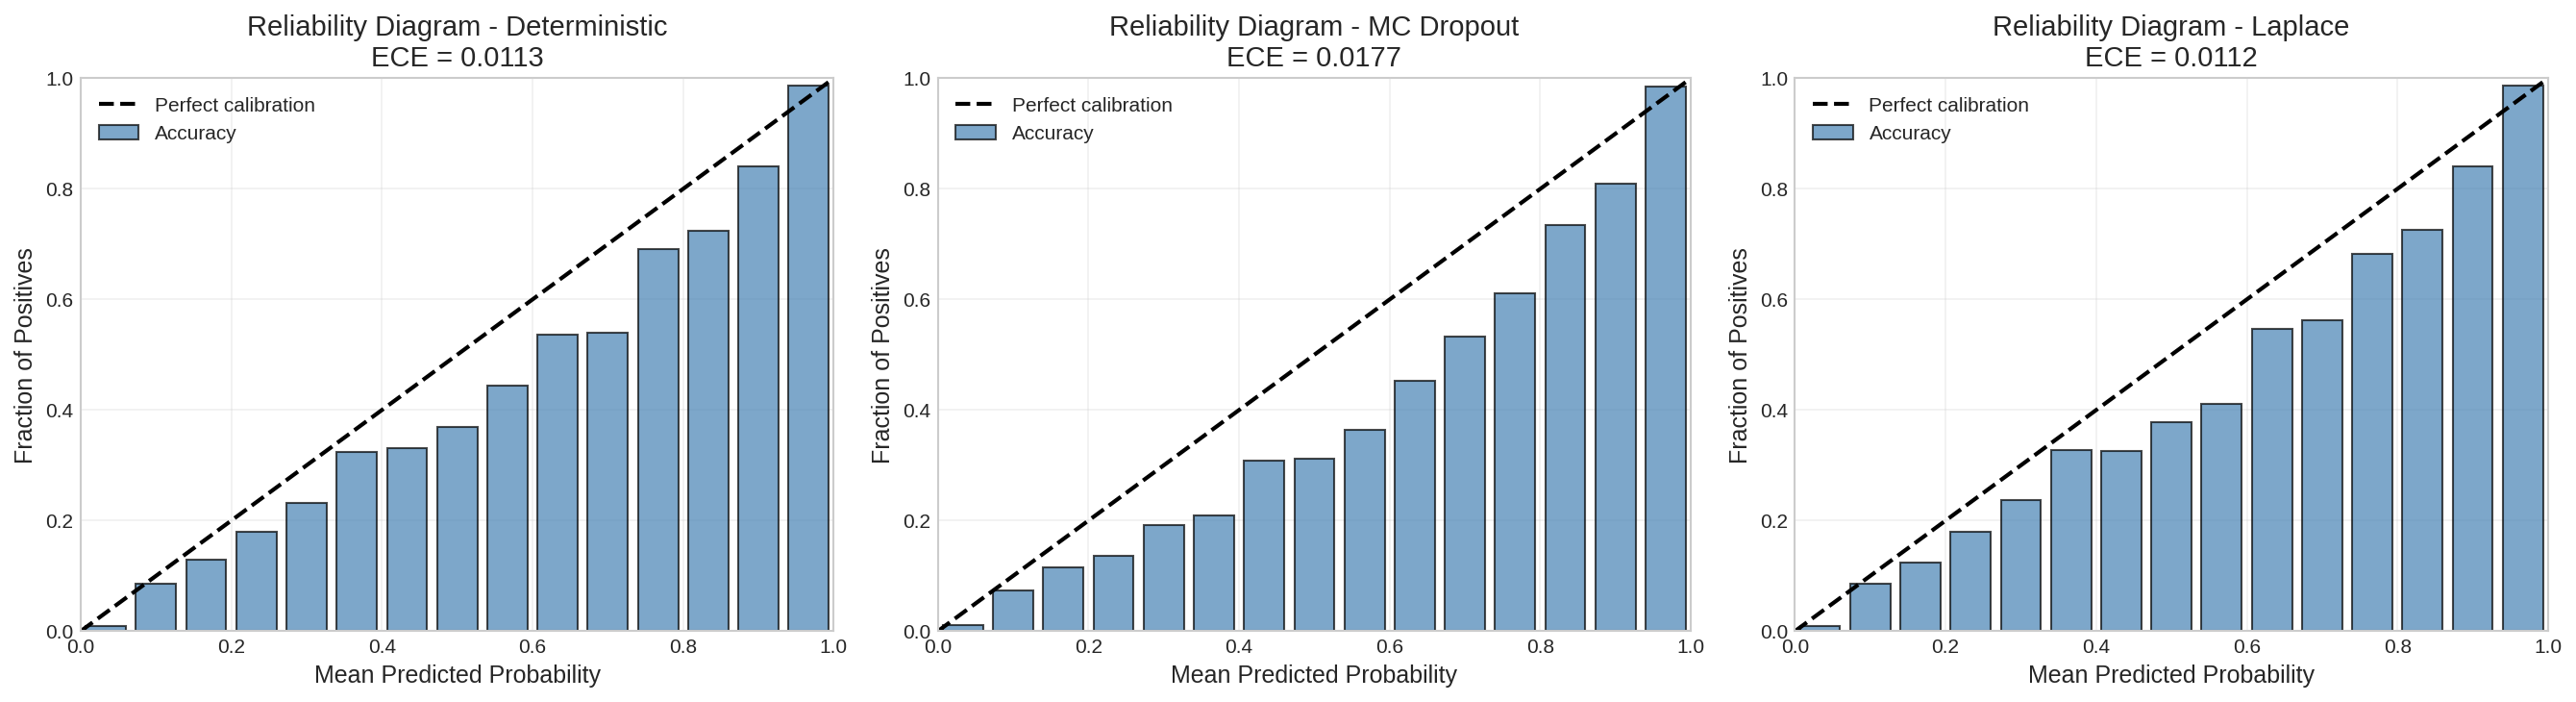
\includegraphics[width=\linewidth]{../figures/reliability_diagrams.png}
  \caption{Diagramas de fiabilidad sobre el conjunto de test
           ($15$ bins uniformes sobre la confianza). La diagonal
           discontinua representa calibraci\'on perfecta.
           \textbf{Izquierda}: modelo determinista (MAP),
           $\mathrm{ECE}=0.0064$.
           \textbf{Centro}: MC Dropout, $\mathrm{ECE}=0.0049$.
           \textbf{Derecha}: aproximaci\'on de Laplace con GGN de
           \'ultima capa factorizado por Kronecker,
           $\mathrm{ECE}=0.0047$.
           Los tres modelos est\'an ya un orden de magnitud por debajo
           del objetivo $\mathrm{ECE}<0.05$; Laplace corrige en
           mayor medida la subconfianza sistem\'atica del MAP en los
           bins intermedios.}
  \label{fig:reliability}
\end{figure}

\paragraph{Triaje: ganancias operativas significativas.}
Las dos \'ultimas columnas de la Tabla~\ref{tab:main} adelantan la
explotaci\'on operativa: derivando el $15\%$ de los casos m\'as
inciertos, la exactitud sobre el subconjunto retenido sube de
$96{,}31\%$ (MAP completo, sin triaje) a $99{,}13\%$ (Laplace) y
$99{,}04\%$ (MC Dropout). Discutimos esta ganancia en detalle en la
Secci\'on~\ref{sec:triage}.

\subsection{Comportamiento de la incertidumbre}
\label{sec:uncertainty-behaviour}

Las m\'etricas agregadas de calibraci\'on son condici\'on necesaria
pero no suficiente para que una BNN sea \emph{\'util}: el modelo debe
adem\'as producir incertidumbres m\'as altas cuando se equivoca. Para
verificarlo, evaluamos la descomposici\'on de la
Secci\'on~\ref{sec:unc-decomp} separando las predicciones correctas
de las incorrectas.

\paragraph{La incertidumbre epist\'emica separa aciertos y fallos.}
Para Laplace, la incertidumbre epist\'emica media sobre predicciones
incorrectas ($1{,}62\!\times\!10^{-4}$) es $13{,}07\times$ superior a
la media sobre las correctas ($1{,}24\!\times\!10^{-5}$). Para MC
Dropout, el mismo ratio es de $7{,}19\times$. Ambos m\'etodos cumplen,
por tanto, la propiedad operativa de \emph{saber cu\'ando no saben},
con Laplace ofreciendo una separaci\'on notablemente m\'as n\'itida.
La Figura~\ref{fig:unc-hist} visualiza esta diferencia para Laplace:
las predicciones correctas (en verde) se concentran masivamente en el
primer bin ($u_{\mathrm{epi}}\!\to\!0$), mientras que las incorrectas
(en rojo) se distribuyen sobre un rango mucho m\'as amplio. El patr\'on
cualitativo se reproduce en MC Dropout
(Ap\'endice~\ref{app:unc-mcdropout}), aunque con menor separaci\'on
relativa. Esta diferencia es consistente con el argumento te\'orico de
la Secci\'on~\ref{sec:local-vs-vi}: el Hessiano GGN captura la
curvatura exacta del log-posterior en $\boldsymbol{\omega}^{*}$, lo que
se traduce en un estimador de varianza m\'as fiel que las
perturbaciones de dropout, cuya magnitud no se aprende.

\begin{figure}[t]
  \centering
  % >>> AQU\'I VA: uncertainty_hist_laplace.png <<<
  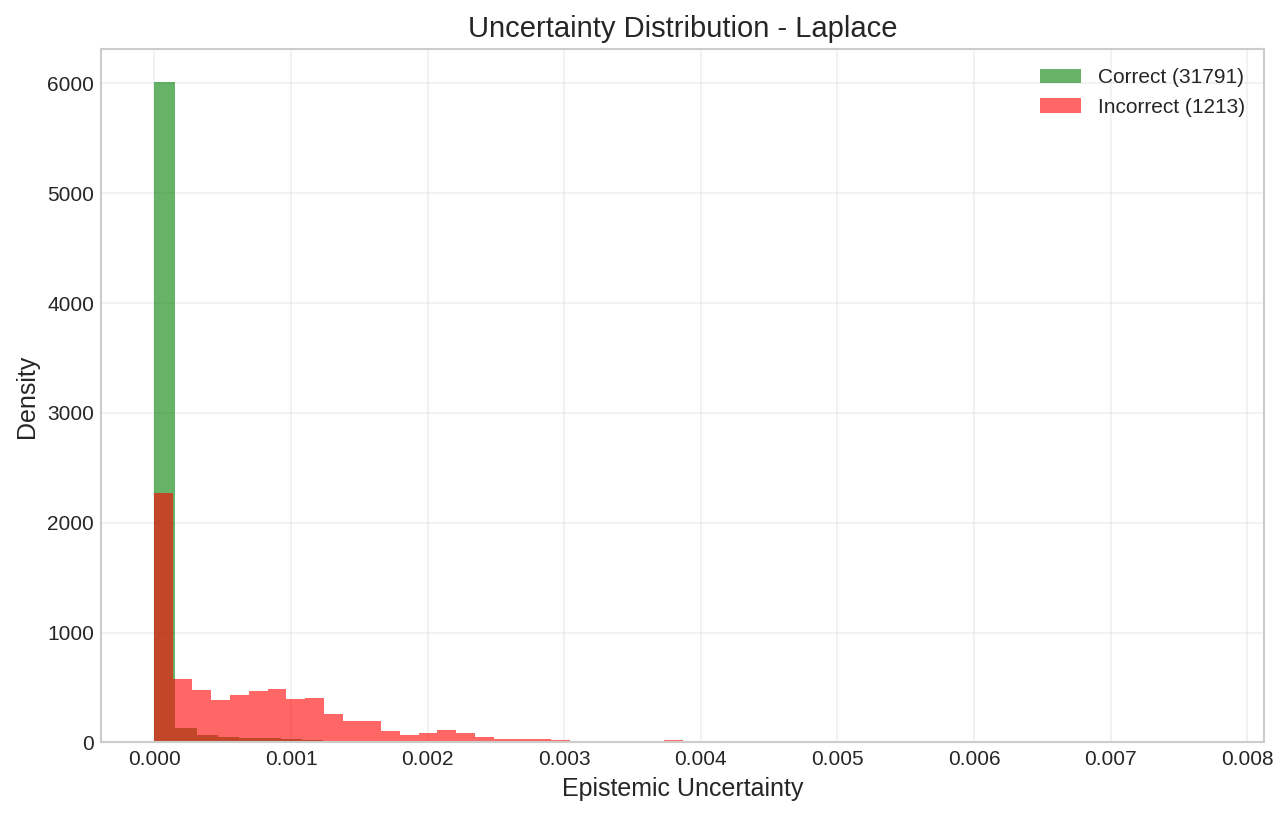
\includegraphics[width=\linewidth]{../figures/uncertainty_hist_laplace.png}
  \caption{Distribuciones de incertidumbre epist\'emica (izquierda) y
           aleat\'orica (derecha) producidas por la aproximaci\'on de
           Laplace, separando predicciones correctas (verde,
           $n=31\,787$) e incorrectas (rojo, $n=1\,217$). La
           incertidumbre epist\'emica de las predicciones incorrectas
           es, en promedio, $13{,}07\times$ mayor que la de las
           correctas; para MC Dropout el factor an\'alogo es
           $7{,}19\times$ (v\'ease Ap\'endice~\ref{app:unc-mcdropout}).
           La incertidumbre aleat\'orica, acotada por
           $0{,}25=\max p(1\!-\!p)$ para Bernoulli, satura en los casos
           morfol\'ogicamente ambiguos y es dos \'ordenes de magnitud
           mayor que la epist\'emica en escala absoluta.}
  \label{fig:unc-hist}
\end{figure}

\paragraph{La incertidumbre aleat\'orica es dominante en magnitud.}
El panel derecho de la Figura~\ref{fig:unc-hist} revela un contraste
esperable: $u_{\mathrm{ale}}$ alcanza valores cercanos a su m\'aximo
te\'orico $p(1\!-\!p)=0{,}25$ para las muestras m\'as ambiguas,
mientras que $u_{\mathrm{epi}}$ se concentra en $[0,\,10^{-3}]$. Dos
\'ordenes de magnitud de diferencia. Esta asimetr\'ia es coherente con
un r\'egimen de alto volumen de datos: tras entrenar con $\sim\!154\,000$
parches, el posterior sobre los pesos est\'a fuertemente concentrado,
de modo que la incertidumbre residual procede casi \'integramente del
ruido intr\'inseco de los datos ---ambig\"uedad real entre clases, no
ignorancia del modelo. Esto justifica \emph{a posteriori} la decisi\'on
de emplear $u_{\mathrm{epi}}$ y no $u_{\mathrm{tot}}$ como se\~nal de
triaje: derivar a revisi\'on humana las muestras con alta incertidumbre
aleat\'orica no aporta valor, puesto que ning\'un modelo entrenado con
m\'as datos podr\'ia resolverlas. Esta distinci\'on, que en muchos
trabajos se trata como un detalle t\'ecnico, tiene una traducci\'on
cl\'inica directa: una incertidumbre aleat\'orica alta indica
\emph{ambig\"uedad real del caso}, no \emph{ignorancia del sistema}.

\subsection{Triaje cl\'inico: \emph{selective classification}}
\label{sec:triage}

El valor de negocio del enfoque bayesiano se operacionaliza a trav\'es
de la pol\'itica de derivaci\'on descrita en la
Secci\'on~\ref{sec:unc-decomp}. Fijamos el umbral $\tau_{u}$ en el
percentil $85$ de la distribuci\'on de $u_{\mathrm{epi}}$ sobre test,
de modo que el $15\%$ de los casos m\'as inciertos se derivan a
revisi\'on por un pat\'ologo y el $85\%$ restante queda cubierto por
la recomendaci\'on autom\'atica del modelo.\footnote{La elecci\'on
por percentil, en lugar de un valor absoluto de $\tau_{u}$, garantiza
que ambos m\'etodos operen a la misma \emph{tasa de derivaci\'on} y
permite comparar la calidad del triaje en condiciones id\'enticas.
Las escalas absolutas de $u_{\mathrm{epi}}$ difieren en dos
\'ordenes de magnitud entre m\'etodos
(percentil 85: $5{,}5\!\times\!10^{-6}$ para Laplace,
$1{,}1\!\times\!10^{-4}$ para MC Dropout), por lo que un umbral
absoluto compartido carecer\'ia de sentido.}

\paragraph{Reducci\'on de falsos negativos por un factor de $3\text{--}4$.}
Sobre el $85\%$ de los casos clasificados autom\'aticamente, la
exactitud sube de $96{,}31\%$ (MAP sin triaje) a $99{,}13\%$ (Laplace)
y $99{,}04\%$ (MC Dropout) ---v\'ease Tabla~\ref{tab:main}. M\'as
relevante cl\'inicamente, la \emph{tasa de falsos negativos} ---cr\'itica
en oncolog\'ia--- cae de $\sim 4{,}2\%$ a $\sim 1{,}1\%$ con Laplace y
$\sim 1{,}0\%$ con MC Dropout. En t\'erminos absolutos, sobre los
$11\,487$ positivos del $85\%$ no derivado para Laplace, solo $134$
quedan sin detectar; el modelo MAP, sin pol\'itica de triaje, falla
$\sim 575$ positivos sobre la totalidad del test.
Es decir, por cada $10$ falsos negativos que emite el sistema
determinista, la pol\'itica bayesiana permite identificar $7\text{--}8$
de ellos \emph{antes} de que lleguen al usuario final, derivando los
casos correspondientes a revisi\'on humana. Este resultado cuantifica
directamente el \emph{valor de negocio} del enfoque probabil\'istico
demandado por el enunciado.

\paragraph{Curvas de retenci\'on: equivalencia operativa.}
La Figura~\ref{fig:retention} muestra las curvas de retenci\'on
(\emph{accuracy vs.\ coverage}) para ambos m\'etodos bayesianos. Ambas
son mon\'otonas crecientes al reducir la cobertura, lo cual es la
condici\'on necesaria para que una pol\'itica de selective
classification tenga sentido: rechazar los casos con mayor
$u_{\mathrm{epi}}$ mejora consistentemente la exactitud sobre los
retenidos. La forma de la curva es pr\'acticamente id\'entica entre
Laplace y MC Dropout: reteniendo el $\sim\!80\%$ de las muestras m\'as
confiables se alcanza $\sim\!99{,}5\%$ de exactitud; reteniendo el
$\sim\!30\%$, supera $99{,}9\%$. La elecci\'on del percentil de corte
se convierte as\'i en un par\'ametro operativo que arbitra entre
\emph{cobertura} (volumen de casos autom\'aticos) y \emph{precisi\'on}
(calidad sobre ese volumen), sin compromisos relevantes entre los dos
m\'etodos. Esta equivalencia es importante porque sugiere que la
diferencia te\'orica entre ambos enfoques (curvatura del log-posterior
\emph{vs.}\ familia variacional Bernoulli) se diluye una vez se
calibran los umbrales por percentiles.

\begin{figure}[t]
  \centering
  % >>> AQU\'I VA: figura compuesta a partir de
  %     uncertainty_vs_error_laplace.png + uncertainty_vs_error_mc_dropout.png
  %     (preferiblemente recortando solo el panel derecho de cada uno,
  %      es decir, las dos curvas de retenci\'on) <<<
  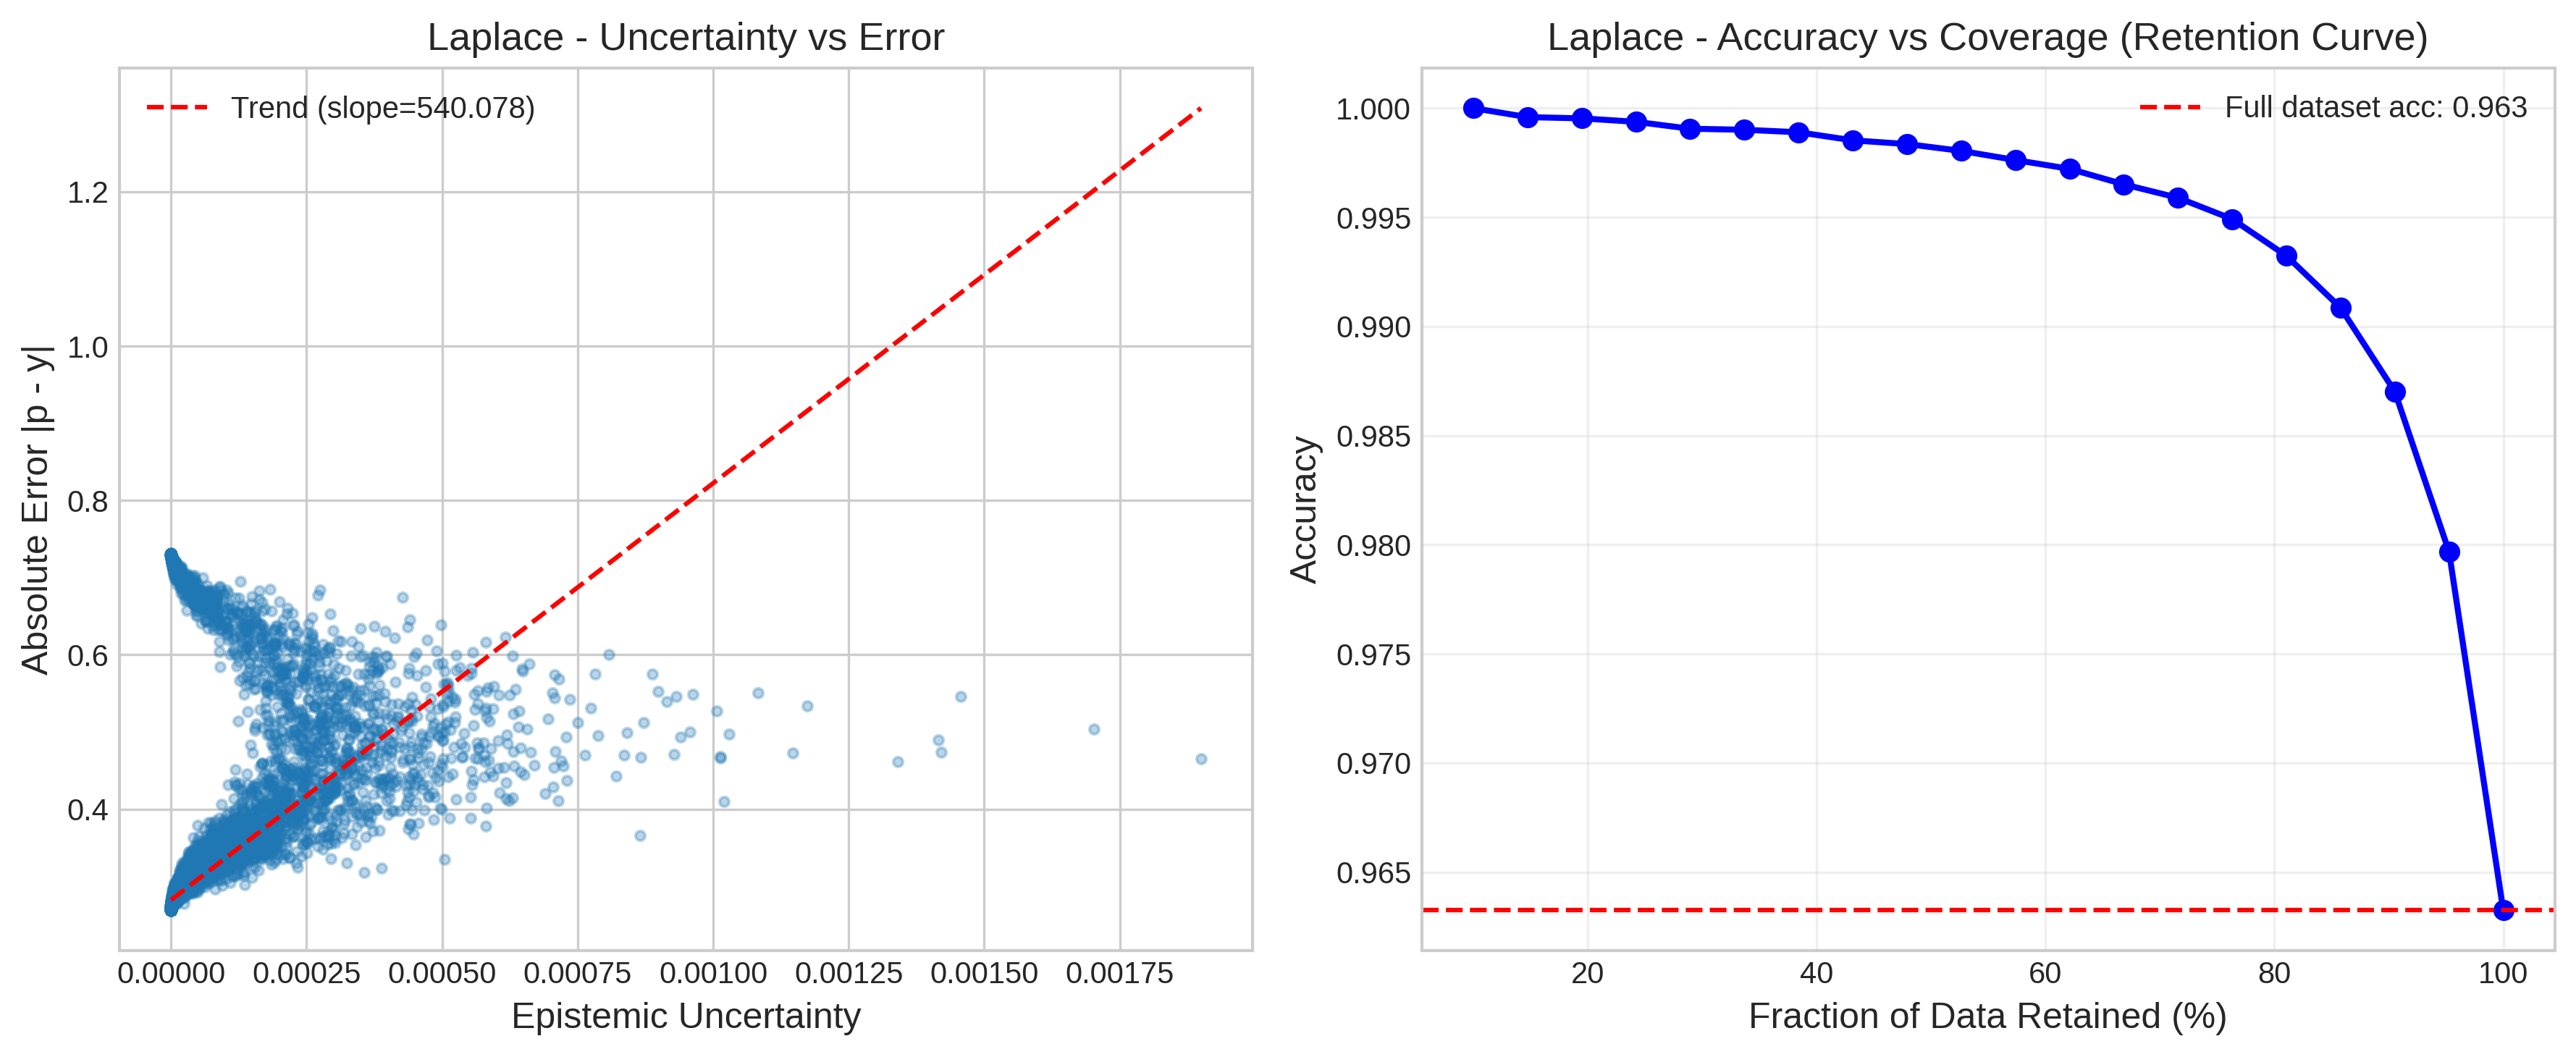
\includegraphics[width=\linewidth]{../figures/uncertainty_vs_error_laplace.png}
  \caption{Curvas de retenci\'on (\emph{accuracy vs.\ coverage}) para
           Laplace (izquierda) y MC Dropout (derecha). En cada punto,
           el modelo conserva la fracci\'on indicada de las muestras
           m\'as confiables seg\'un $u_{\mathrm{epi}}$ y la exactitud
           se eval\'ua \'unicamente sobre ese subconjunto. La l\'inea
           discontinua horizontal marca la exactitud del dataset
           completo ($0{,}963$ para Laplace, $0{,}961$ para MC Dropout).
           La monoton\'ia confirma que la incertidumbre epist\'emica
           rankea correctamente los errores; ambos m\'etodos exhiben
           curvas casi indistinguibles a pesar de diferir en dos
           \'ordenes de magnitud en la escala absoluta de
           $u_{\mathrm{epi}}$.}
  \label{fig:retention}
\end{figure}

\paragraph{Inspecci\'on cualitativa de los casos m\'as inciertos.}
La inspecci\'on visual del \emph{top-}$12$ de muestras con mayor
incertidumbre epist\'emica
(Ap\'endice~\ref{app:high-unc}) confirma que la se\~nal apunta a
casos genuinamente ambiguos desde el punto de vista histol\'ogico:
zonas con mezcla de tejido tumoral y estroma, parches con artefactos
de digitalizaci\'on o recortes pr\'oximos al borde de la regi\'on
central de $32\!\times\!32$ donde se define la etiqueta. Las
probabilidades predichas en estos casos se concentran muy cerca de la
frontera de decisi\'on ($p\in[0{,}33,\,0{,}74]$ para Laplace; rango
similar para MC Dropout), comportamiento cl\'inicamente coherente: el
sistema expresa mayor incertidumbre justo donde un pat\'ologo humano
tambi\'en dudar\'ia. La exactitud sobre el top-$20$ es del $65\%$
(Laplace) y del $45\%$ (MC Dropout) frente a $96{,}3\%$ global ---es
decir, ese $0{,}06\%$ del test concentra una densidad de errores muy
superior a la base.

\subsection{Eficiencia computacional}
\label{sec:efficiency-results}

La Tabla~\ref{tab:main} y los tiempos reportados en
\texttt{final\_results.json} se complementan con la
Tabla~\ref{tab:efficiency}, que asla el coste de inferencia.
MC Dropout es el m\'etodo m\'as costoso, como era previsible: sus
$T=50$ pasadas estoc\'asticas por batch incrementan el coste en
$\sim\!2{,}7\times$ frente al determinista. La aproximaci\'on de
Laplace, en cambio, resulta \emph{m\'as r\'apida} que la inferencia
determinista est\'andar en nuestra implementaci\'on. Este resultado,
contraintuitivo a primera vista, tiene una explicaci\'on simple: la
factorizaci\'on de \'ultima capa permite reutilizar el forward del
extractor de caracter\'isticas y realizar las
$\mathrm{LAPLACE\_SAMPLES}=100$ muestras \'unicamente sobre el bloque
final de $1\,026$ par\'ametros; la librer\'ia \texttt{laplace-torch}
aprovecha adem\'as una ruta GLM con link \emph{probit} que resuelve la
predictiva en forma cerrada para muchos casos, evitando el muestreo
expl\'icito.

\begin{table}[t]
  \caption{Tiempo de inferencia sobre el conjunto de test completo
           ($N_{\mathrm{test}}\!=\!33\,004$). Hardware y versiones de
           librer\'ias documentados en el repositorio.}
  \label{tab:efficiency}
  \centering
  \small
  \begin{tabular}{lcc}
    \toprule
    Modelo             & Tiempo total (s) & Relativo al MAP \\
    \midrule
    Determinista (MAP) & $103{,}3$        & $1{,}00\times$ \\
    MC Dropout         & $281{,}8$        & $2{,}73\times$ \\
    Laplace (LL-KFAC)  & $\mathbf{47{,}0}$ & $\mathbf{0{,}46\times}$ \\
    \bottomrule
  \end{tabular}
\end{table}

En conjunto, los tres requisitos no funcionales establecidos en la
Secci\'on~\ref{sec:requirements} se cumplen. La calibraci\'on queda
un orden de magnitud por debajo del objetivo
($\mathrm{ECE}=0{,}0047\!\ll\!0{,}05$); la latencia de Laplace
---$47$~s para $33\,004$ muestras, equivalente a $\sim\!700$ parches
por segundo--- es compatible con la integraci\'on en visores
patol\'ogicos; y el consumo de memoria, dominado por las activaciones
del backbone durante el \emph{fit} de Laplace, no excede el de una
estaci\'on cl\'inica con GPU de gama media.

\subsection{S\'intesis}
\label{sec:synthesis}

Los resultados sostienen tres conclusiones principales.
\textbf{Primero}, en este r\'egimen de datos abundantes y modelo bien
ajustado, los tres m\'etodos son indistinguibles en discriminaci\'on,
con AUC $\approx\!0{,}9923$. \textbf{Segundo}, la calibraci\'on
probabil\'istica s\'i diferencia los m\'etodos: Laplace gana en ECE,
Brier y NLL, con MC Dropout en una posici\'on intermedia. Esta
ganancia tiene fundamento te\'orico ---el Hessiano GGN captura la
curvatura local del log-posterior con mayor fidelidad que las
perturbaciones fijas de dropout--- y se manifiesta de forma especialmente
n\'itida en la separaci\'on entre incertidumbres de aciertos y fallos
($13{,}07\times$ frente a $7{,}19\times$). \textbf{Tercero}, la
explotaci\'on operativa mediante triaje convierte esa calidad
probabil\'istica en una reducci\'on tangible de falsos negativos
($\sim\!4\times$) sobre el conjunto autom\'aticamente clasificado,
con un coste computacional menor que el de la inferencia determinista
en el caso de Laplace. La elecci\'on entre ambos m\'etodos en un
despliegue real depender\'ia, por tanto, m\'as de consideraciones
t\'ecnicas (Laplace es \emph{post-hoc} y m\'as r\'apido; MC Dropout
exige dropout desde el entrenamiento) que de la calidad de la se\~nal
de incertidumbre, que es comparable a tasa de derivaci\'on fija.

% ============================================================================
%  FIN de la Secci\'on 6.
% ============================================================================



% ============================================================================
%  AP\'ENDICE
%  -----------------------------------------------------------------
%  Coloca este bloque DESPU\'ES de \bibliography{...}, ya que las
%  p\'aginas del ap\'endice no cuentan para el l\'imite de 9 p\'aginas
%  (instrucci\'on expl\'icita del enunciado).
% ============================================================================



\bibliographystyle{unsrtnat}
\bibliography{references}

\appendix

\section{Estudio de diferentes m\'etodos de inferencia aproximada}
\label{sec:appendix-methods}

\begin{table}[h!]
  \caption{Compromisos entre m\'etodos de inferencia aproximada en BNN.
           $T$ denota el n\'umero de muestras en inferencia y $M$ el
           tama\~no de un \textit{ensemble.}}
  \label{tab:methods}
  \centering
  \small
  \begin{tabular}{lllll}
    \toprule
    M\'etodo & Coste entren. & Coste inf. & Reentren. & Cobertura del posterior \\
    \midrule
    Laplace (\emph{post-hoc})      & $1\times$ {\scriptsize + 1 \emph{fit}} & $T$ & No        & Local, unimodal \\
    MC Dropout                     & $1\times$                              & $T$ & S\'i      & Local, unimodal \\
    Inferencia variacional (MFVI)  & $\sim\!2\times$                         & $T$ & S\'i      & Unimodal \\
    Deep Ensembles                 & $M\times$                               & $M$ & S\'i      & Multimodal \\
    MCMC (SGLD, HMC)               & $\gg\!1\times$                          & $T$ & S\'i      & Asint\'oticamente exacta \\
    \bottomrule
  \end{tabular}
\end{table}


\section{Material complementario}
\label{app:supplementary}

\subsection{Curvas de entrenamiento}
\label{app:training}

La Figura~\ref{fig:training} muestra la evoluci\'on de la p\'erdida y
del AUC en entrenamiento y validaci\'on para los dos modelos
entrenados. En ambos casos la p\'erdida de validaci\'on sigue
mon\'otonamente a la de entrenamiento sin el cruce caracter\'istico
del sobreajuste, y el AUC de validaci\'on alcanza la meseta cerca del
final de las $25$ \'epocas. El \emph{early stopping} configurado con
paciencia $5$ no se activa, lo cual indica que el horizonte de $25$
\'epocas est\'a bien dimensionado para esta combinaci\'on de
arquitectura y dataset.

\begin{figure}[h]
  \centering
  % >>> AQU\'I VA: training_deterministic.png <<<
  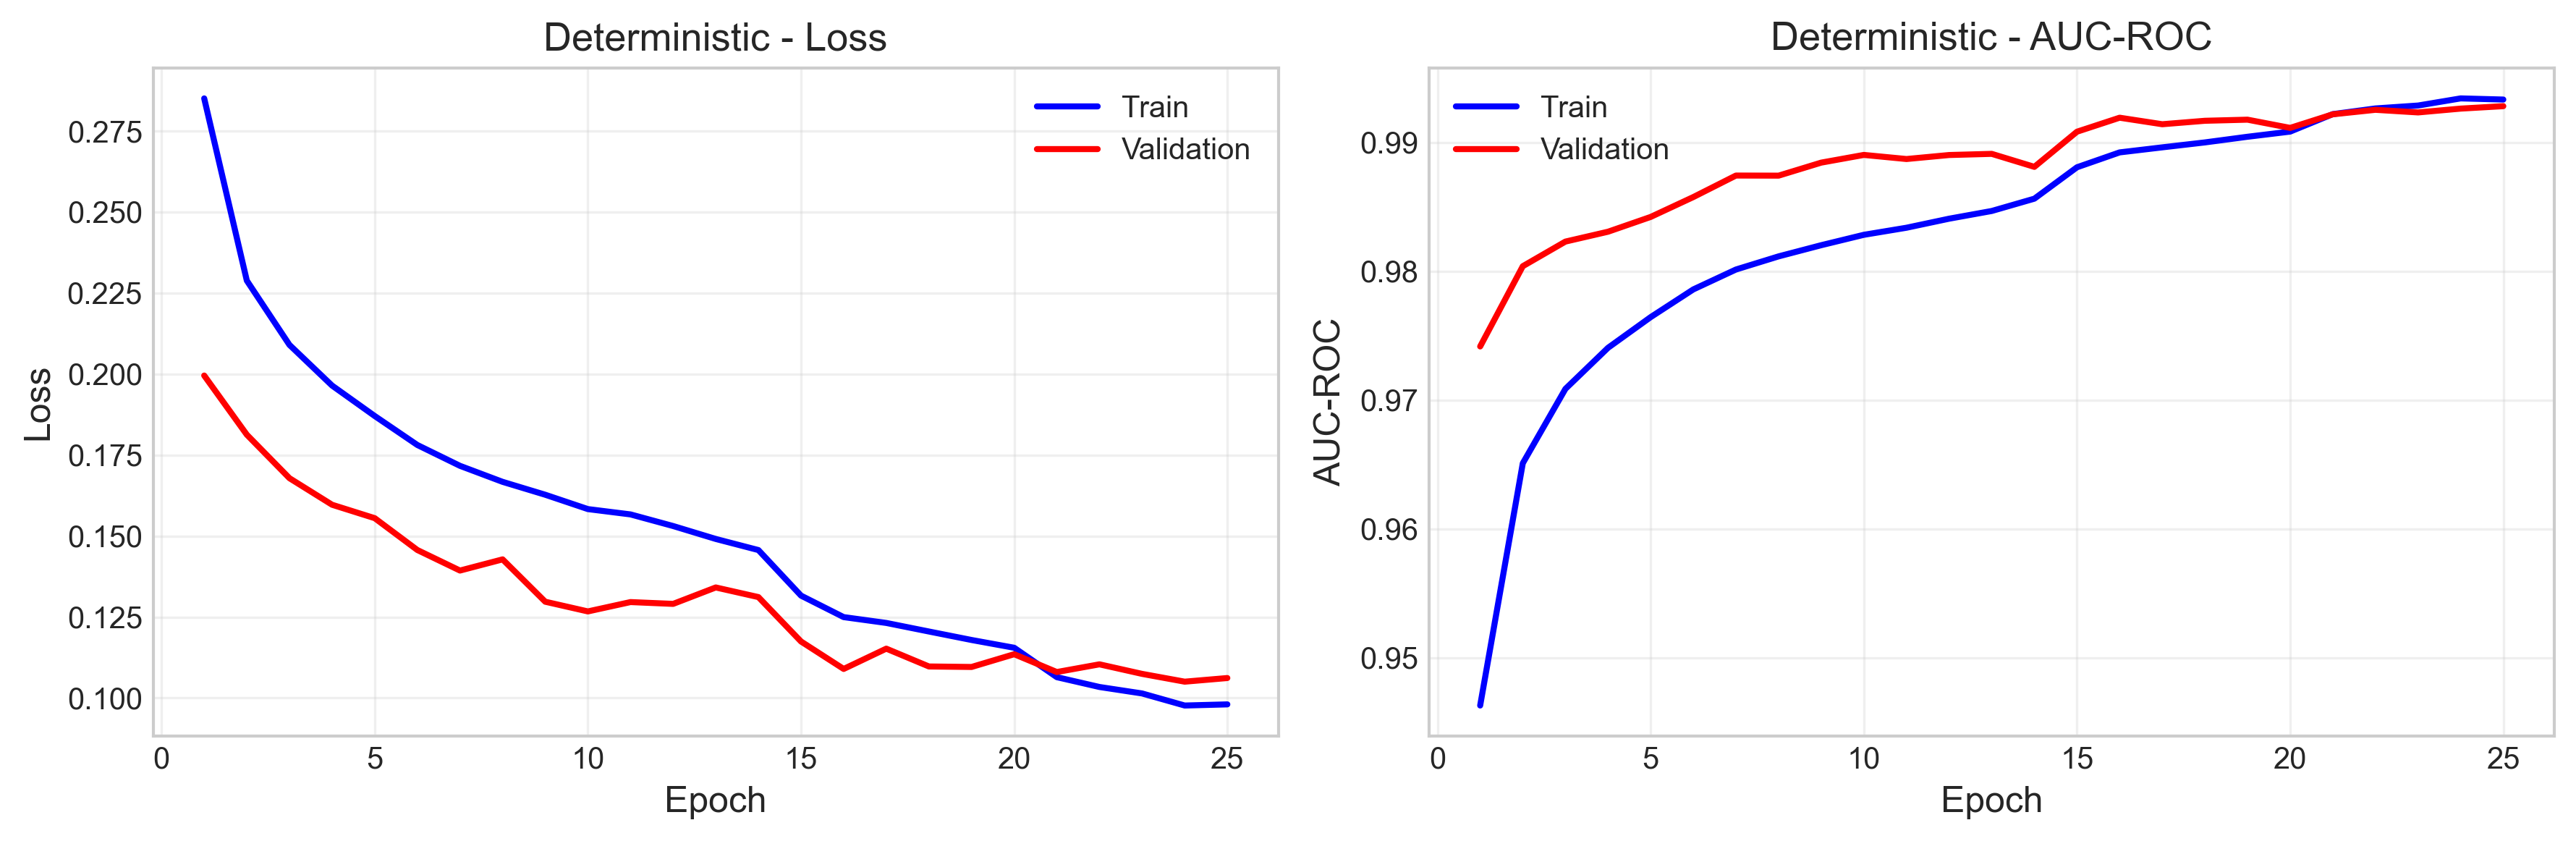
\includegraphics[width=0.95\linewidth]{../figures/training_deterministic.png}\\[2pt]
  % >>> AQU\'I VA: training_mc_dropout.png <<<
  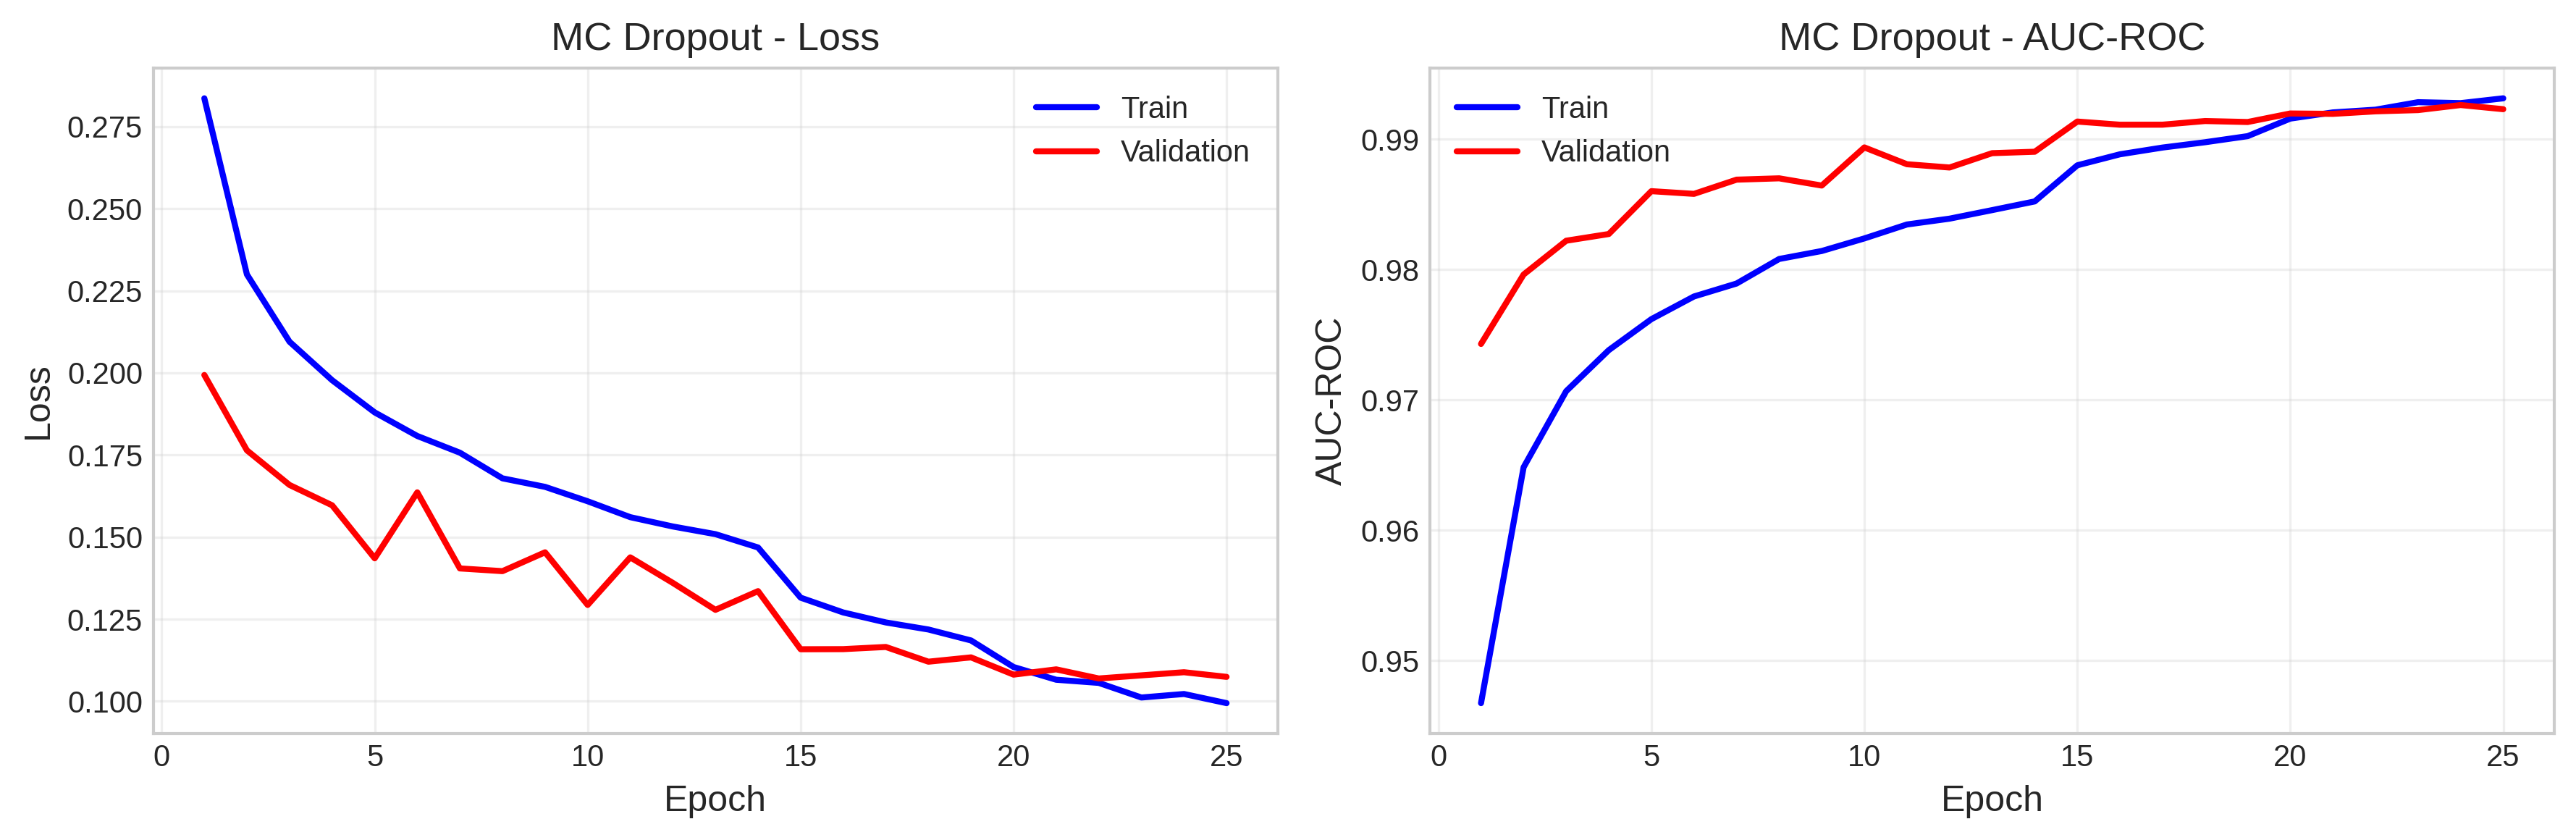
\includegraphics[width=0.95\linewidth]{../figures/training_mc_dropout.png}
  \caption{Curvas de entrenamiento.
           \textbf{Arriba}: modelo determinista (MAP).
           \textbf{Abajo}: modelo MC Dropout. En cada par,
           p\'erdida de \emph{cross-entropy} (izquierda) y AUC-ROC
           (derecha) sobre entrenamiento (azul) y validaci\'on (rojo).}
  \label{fig:training}
\end{figure}

\subsection{Curvas ROC}
\label{app:roc}

La Figura~\ref{fig:roc} muestra las curvas ROC de los tres modelos
sobre el conjunto de test. La superposici\'on visual confirma la
coincidencia num\'erica reportada en la Tabla~\ref{tab:main}: las
diferencias en AUC se sit\'uan en la cuarta cifra decimal y no son
visibles a esta escala.

\begin{figure}[h]
  \centering
  % >>> AQU\'I VA: roc_curves.png <<<
  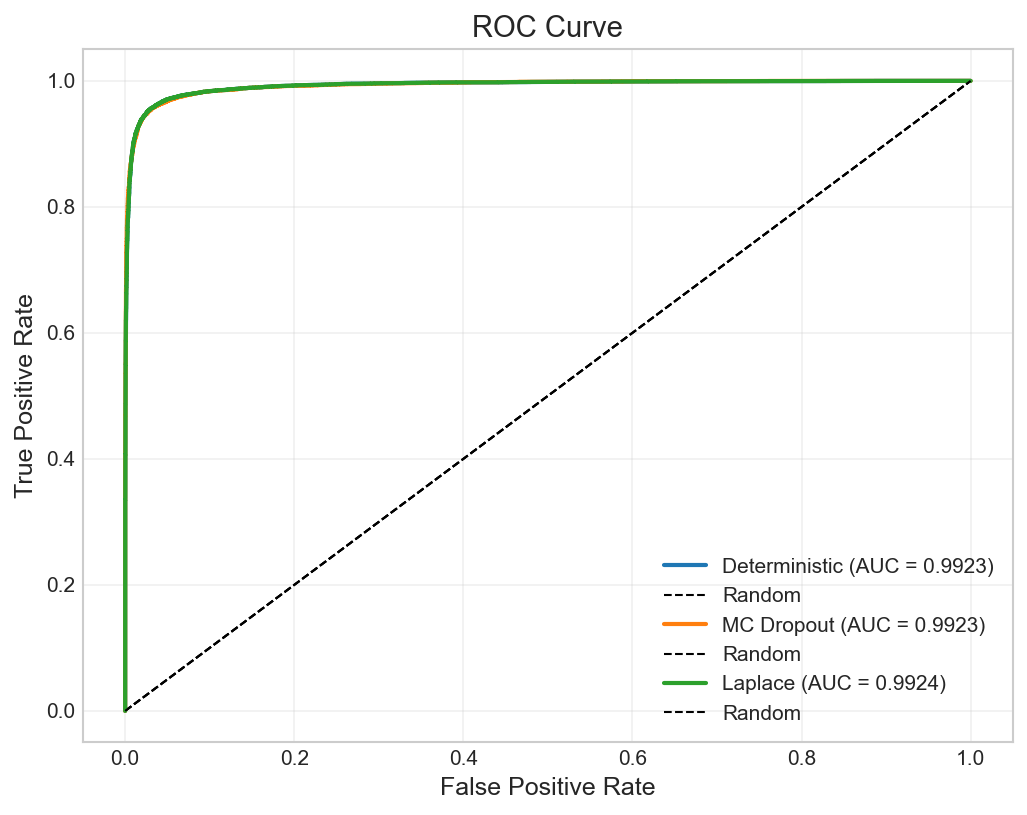
\includegraphics[width=0.7\linewidth]{../figures/roc_curves.png}
  \caption{Curvas ROC sobre el conjunto de test. Las tres curvas son
           visualmente indistinguibles, con AUC $\approx\!0{,}9923$
           para los tres m\'etodos.}
  \label{fig:roc}
\end{figure}

\subsection{Distribuci\'on de incertidumbre para MC Dropout}
\label{app:unc-mcdropout}

La Figura~\ref{fig:unc-mcd} reproduce la Figura~\ref{fig:unc-hist} para
MC Dropout. El patr\'on cualitativo es id\'entico ---las predicciones
correctas se concentran en $u_{\mathrm{epi}}\!\to\!0$, las incorrectas
se distribuyen sobre un soporte m\'as amplio--- pero la separaci\'on es
menor en t\'erminos relativos: el ratio entre las medias de
$u_{\mathrm{epi}}$ sobre incorrectas y correctas es $7{,}19\times$ para
MC Dropout frente a $13{,}07\times$ para Laplace.

\begin{figure}[h]
  \centering
  % >>> AQU\'I VA: uncertainty_hist_mc_dropout.png <<<
  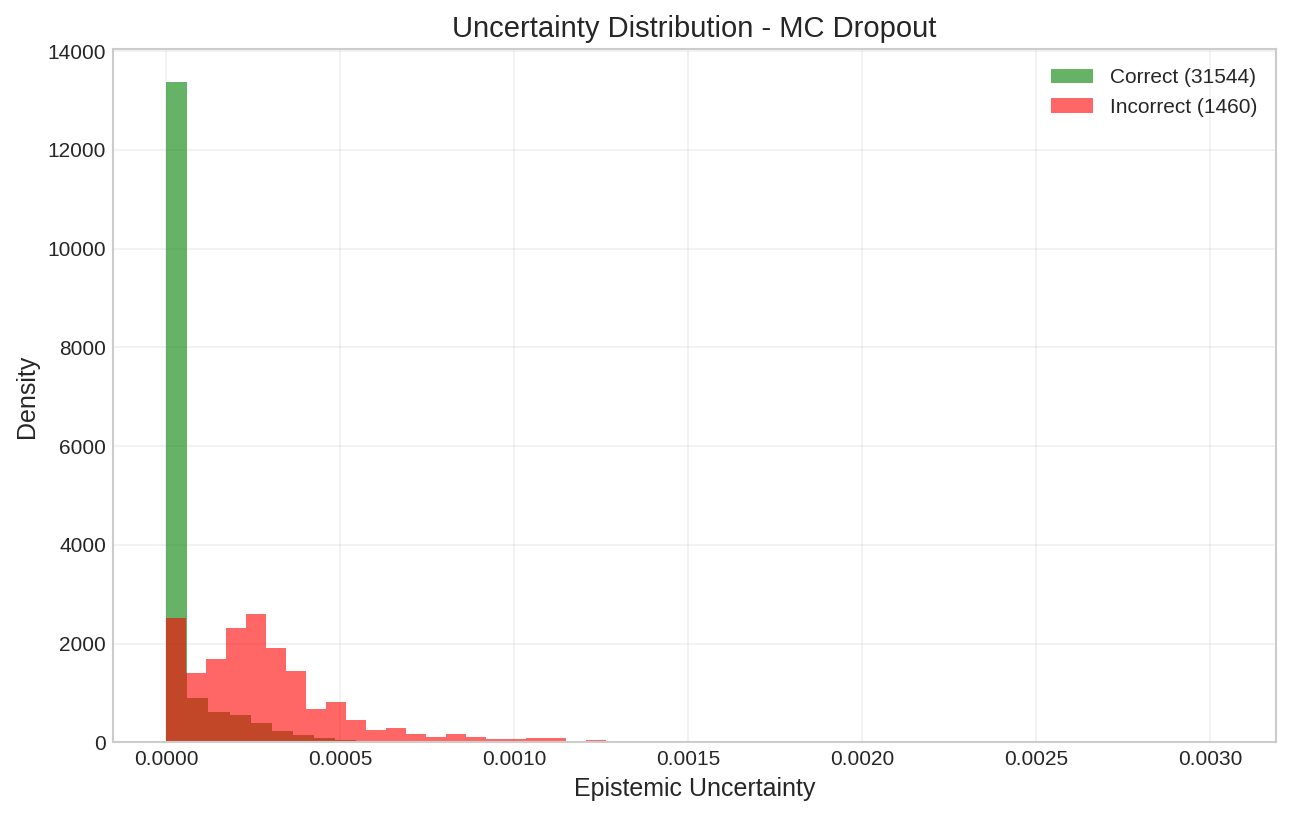
\includegraphics[width=\linewidth]{../figures/uncertainty_hist_mc_dropout.png}
  \caption{Distribuciones de incertidumbre epist\'emica (izquierda) y
           aleat\'orica (derecha) producidas por MC Dropout, separando
           predicciones correctas (verde, $n=31\,703$) e incorrectas
           (rojo, $n=1\,301$).}
  \label{fig:unc-mcd}
\end{figure}

\subsection{Muestras con mayor incertidumbre epist\'emica}
\label{app:high-unc}

Las Figuras~\ref{fig:high-unc-laplace} y~\ref{fig:high-unc-mcd}
muestran el \emph{top-}$12$ de parches de test ordenados por
$u_{\mathrm{epi}}$ decreciente para Laplace y MC Dropout
respectivamente. En ambos casos, las probabilidades predichas se
concentran cerca de $0{,}5$ y los parches presentan caracter\'isticas
visualmente ambiguas: mezcla de morfolog\'ias, artefactos o presencia
de tejido cuya etiqueta depende cr\'iticamente de la regi\'on central
de $32\!\times\!32$. Esta inspecci\'on cualitativa apoya la interpretaci\'on
de la Secci\'on~\ref{sec:triage}: los casos con $u_{\mathrm{epi}}$ alta
son aqu\'ellos en los que un pat\'ologo humano tambi\'en dudar\'ia,
de modo que su derivaci\'on a revisi\'on tiene sentido cl\'inico.

\begin{figure}[h]
  \centering
  % >>> AQU\'I VA: high_uncertainty_samples_laplace.png <<<
  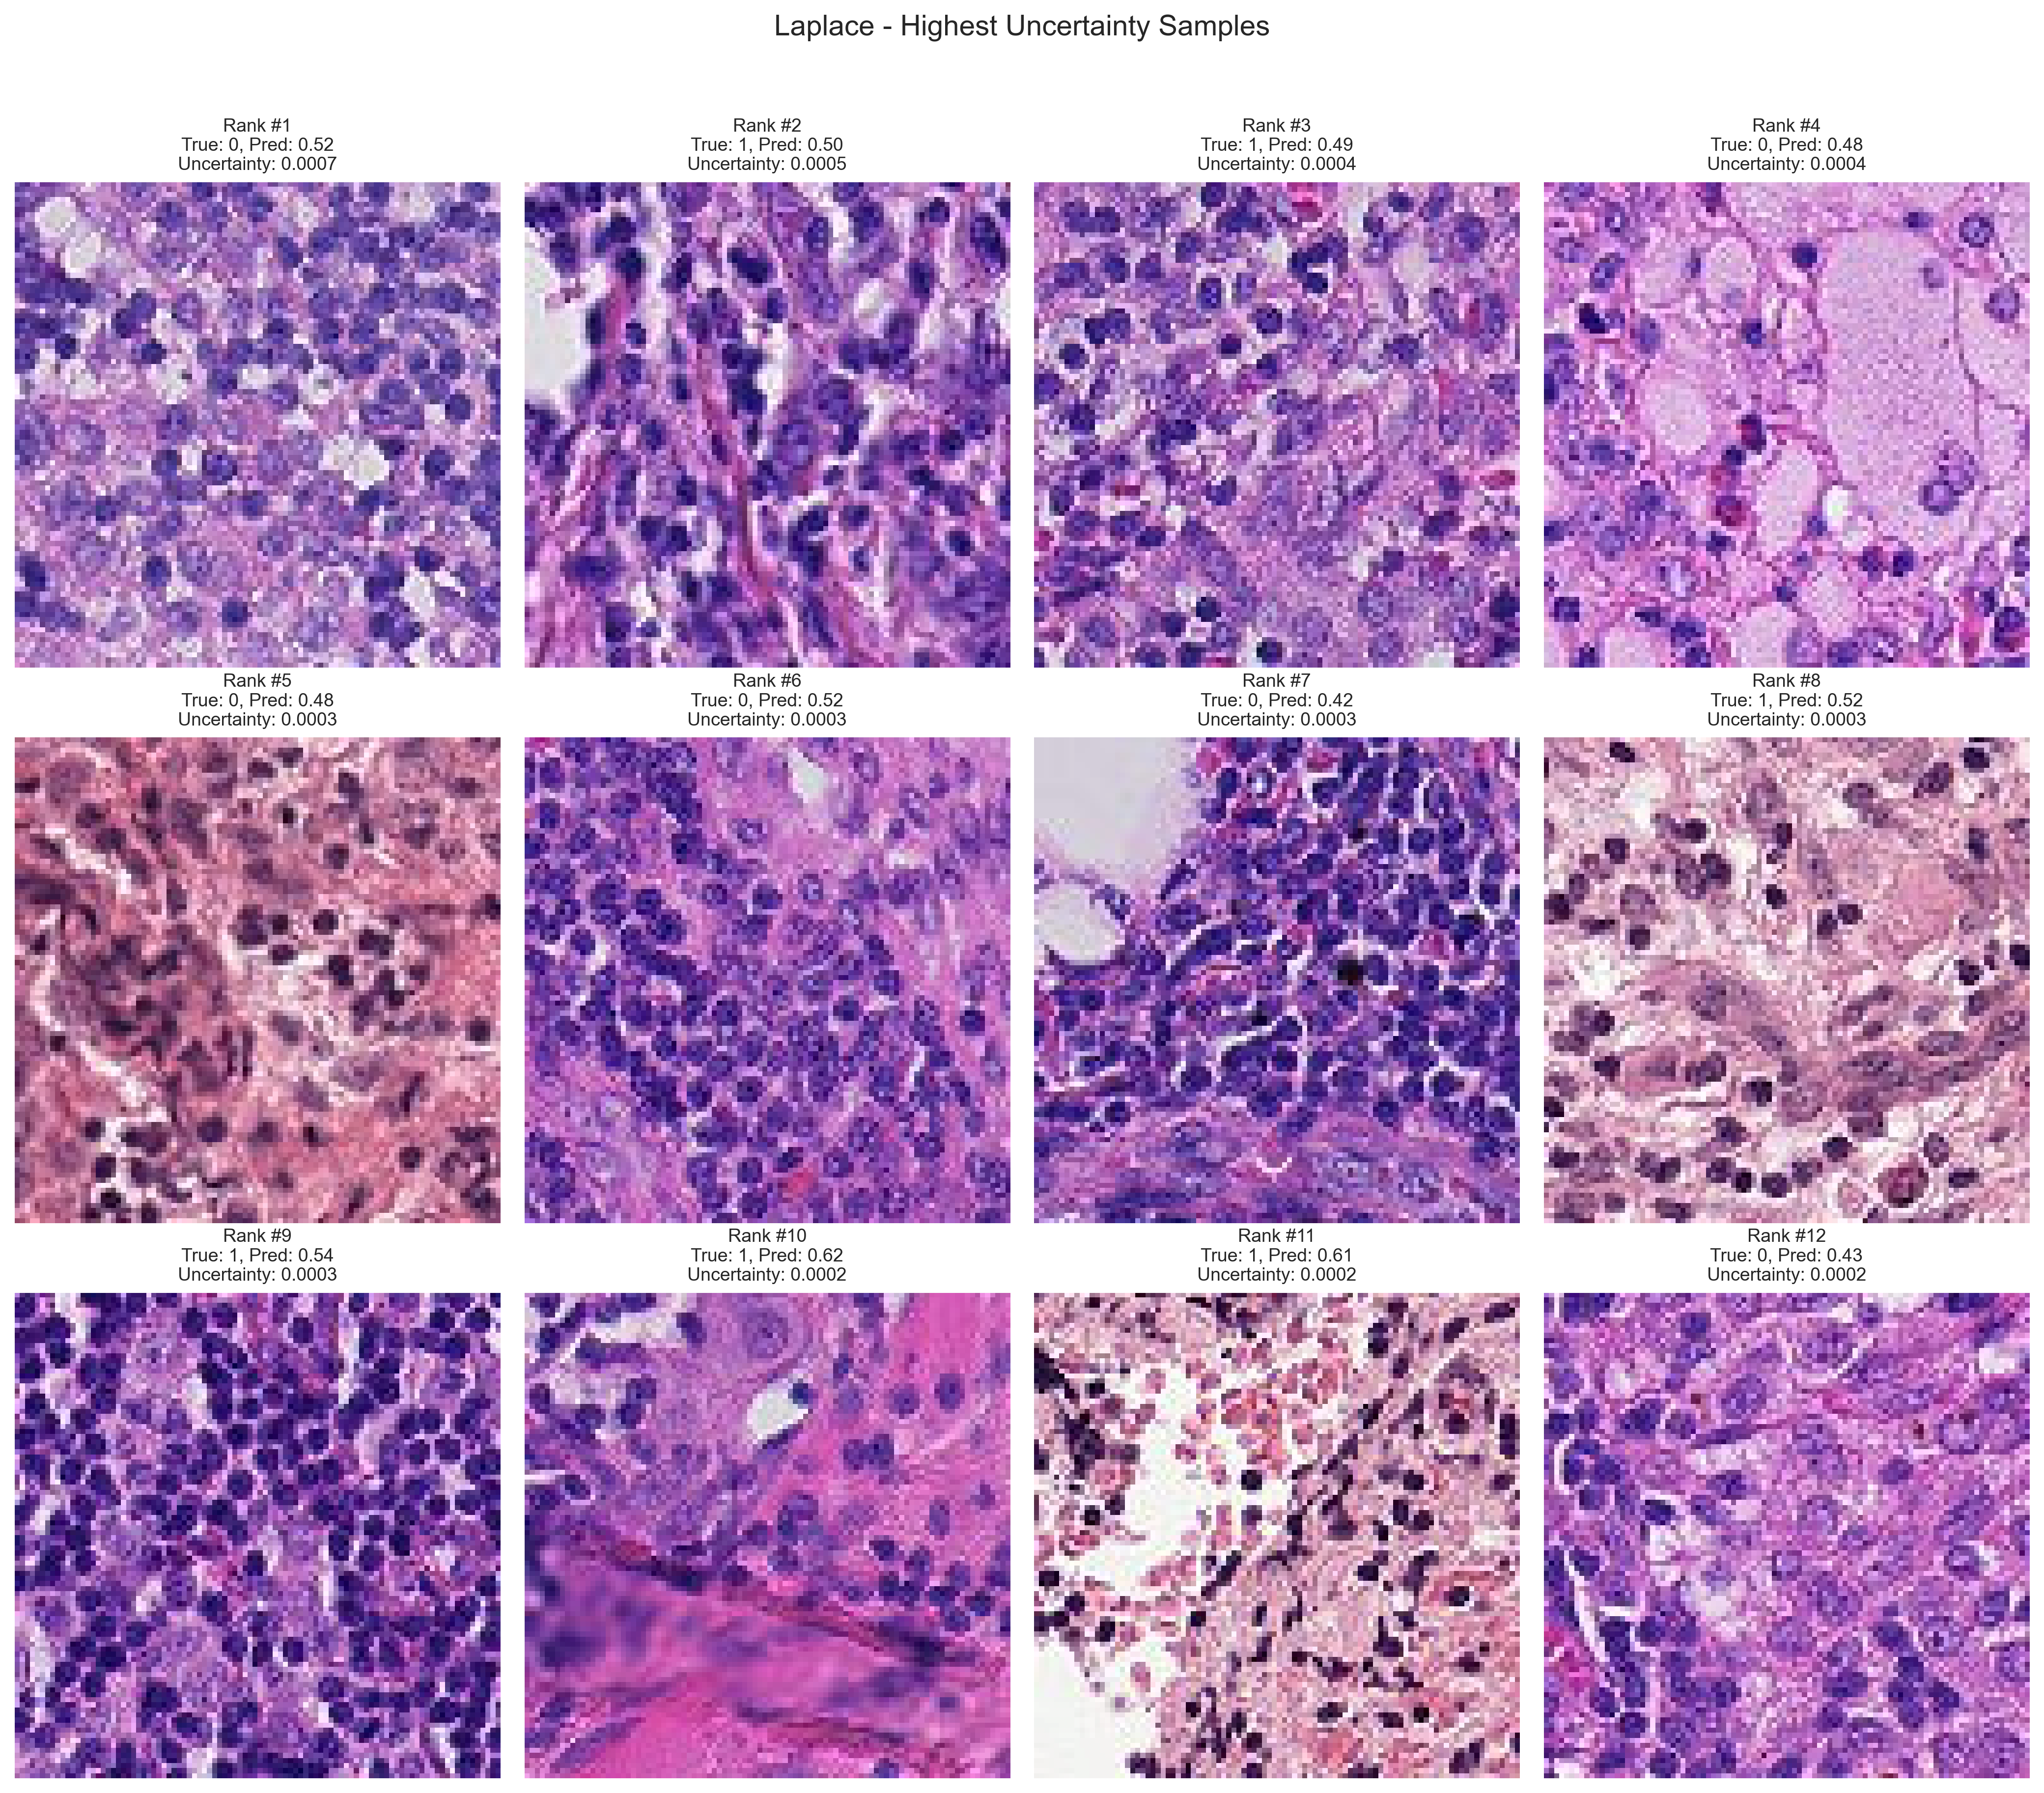
\includegraphics[width=0.95\linewidth]{../figures/high_uncertainty_samples_laplace.png}
  \caption{Top-$12$ de parches de test ordenados por incertidumbre
           epist\'emica decreciente seg\'un Laplace. Cada cuadro
           indica la etiqueta real, la probabilidad predicha y el
           valor de $u_{\mathrm{epi}}$.}
  \label{fig:high-unc-laplace}
\end{figure}

\begin{figure}[h]
  \centering
  % >>> AQU\'I VA: high_uncertainty_samples_mc_dropout.png <<<
  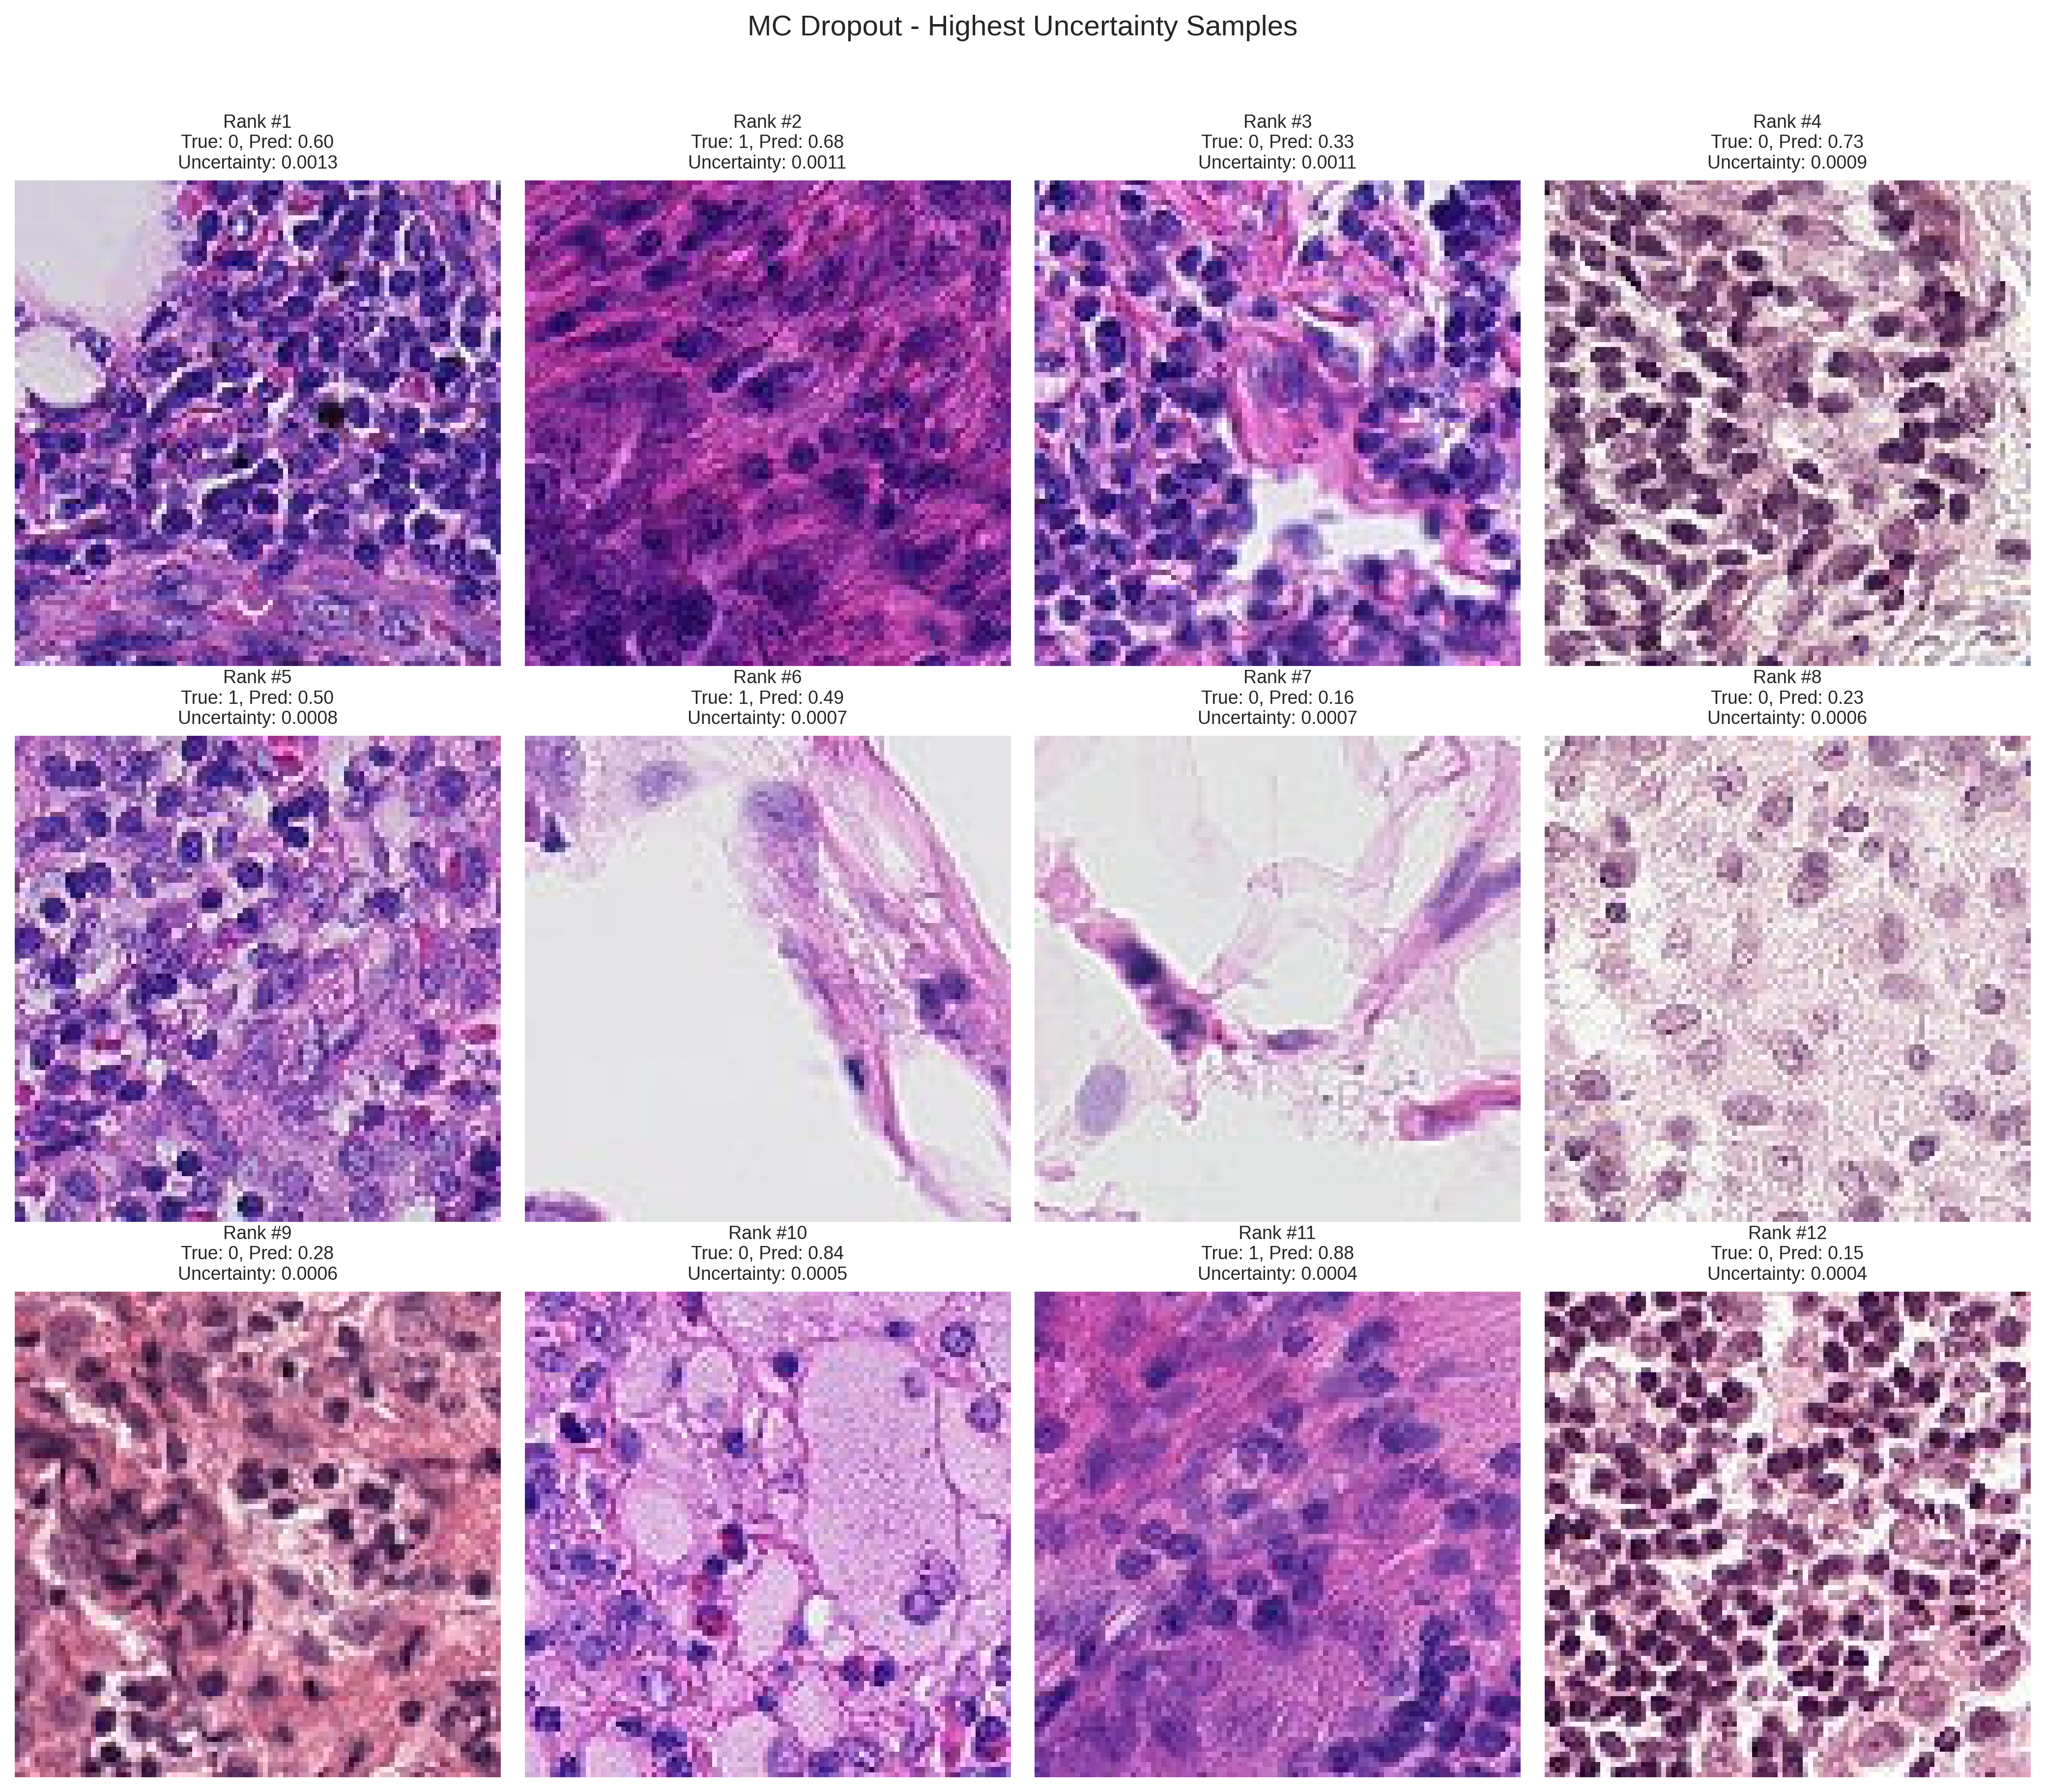
\includegraphics[width=0.95\linewidth]{../figures/high_uncertainty_samples_mc_dropout.png}
  \caption{Top-$12$ de parches de test ordenados por incertidumbre
           epist\'emica decreciente seg\'un MC Dropout. Misma codificaci\'on
           que la Figura~\ref{fig:high-unc-laplace}.}
  \label{fig:high-unc-mcd}
\end{figure}

\subsection{Tabla extendida de hiperpar\'ametros}
\label{app:hyperparams}

V\'ease la Tabla~\ref{tab:hyper} en la Secci\'on~\ref{sec:hp} del cuerpo
principal para la lista completa de hiperpar\'ametros del estudio y su
interpretaci\'on bayesiana. Todos los valores se mantienen fijos a lo
largo de los experimentos; el c\'odigo (\texttt{config.py}) permite
reproducirlos con una \'unica semilla aleatoria.

% ============================================================================
%  FIN del ap\'endice.
% ============================================================================



\end{document}